\documentclass[t, aspectratio=169, table]{_style/izu-beamer}

% ---------------------------------------------------------------
% NOT: babel[turkish] '=' karakterini aktif kısayol yapıp
% includegraphics/tikz/listings key=value sözdizimini bozuyordu.
% Çözüm cls içinde: \usepackage[shorthands=off,turkish]{babel}
% ---------------------------------------------------------------
% Görsel yolu ve kod listeleme paketi
% ---------------------------------------------------------------
\graphicspath{{./}{sekiller/}}

\usepackage{listings}
\lstset{
  language={[ANSI]C},
  basicstyle=\ttfamily\scriptsize,
  keywordstyle=\color{izuBordo}\bfseries,
  commentstyle=\color{izuGold!80!black}\itshape,
  stringstyle=\color{izuDark},
  numberstyle=\tiny\color{izuGrey!60},
  backgroundcolor=\color{izuLightRed!50},
  frame=leftline,
  rulecolor=\color{izuGold},
  framesep=6pt,
  xleftmargin=10pt,
  breaklines=true,
  showstringspaces=false,
  columns=fullflexible,
  keepspaces=true,
}

% ---------------------------------------------------------------
% Sunum meta bilgileri
% ---------------------------------------------------------------
\title[Model Roket Uçuş Bilgisayarı]{Model Roket Uçuş Kontrol Bilgisayarı}
\subtitle{STM32F446 Üzerinde FreeRTOS Tabanlı Aviyonik Yazılım Mimarisi}
\author[H.~Sarıkaya]{Halil Sarıkaya \enspace {\scriptsize 031021037}}
\date{7 Haziran 2026}
\institute{%
  Danışman: Mohammed JOUDA, Dr.~Öğr.~Üyesi\\[1pt]
  Elektrik-Elektronik Mühendisliği\\[1pt]
  İstanbul Sabahattin Zaim Üniversitesi%
}

% ---------------------------------------------------------------
% Başlık sayfasındaki grafik (isteğe bağlı — silmek için yorum satırı)
% ---------------------------------------------------------------
%\titlegraphic{\includegraphics[width=0.35\paperwidth]{sekiller/ornek.pdf}}

% ---------------------------------------------------------------
\begin{document}

% Başlık slaytı
\begin{frame}[plain]
  \titlepage
\end{frame}

% İçindekiler
\begin{frame}{İçindekiler}{}
  \begin{columns}[c]
    \begin{column}{0.5\textwidth}
      \tableofcontents[sections={1-3}]
    \end{column}
    \begin{column}{0.5\textwidth}
      \tableofcontents[sections={4-5}]
    \end{column}
  \end{columns}
\end{frame}

% ---------------------------------------------------------------
% Bölümler ve içerik slaytları
% ---------------------------------------------------------------
% =================================================================
% BÖLÜM 1 — GİRİŞ VE PROBLEM
% =================================================================
\section{Giriş ve Problem}

% ---------------------------------------------------------------
\begin{frame}{Problem ve Motivasyon}{Neden gerçek zamanlı bir uçuş bilgisayarı?}
  \begin{columns}[T]
    \begin{column}{0.52\textwidth}
      \begin{block}{Kritik zaman kısıtı}
        Model roket; fırlatma, serbest uçuş ve \textbf{tepe noktası (apogee)} fazlarını
        \textbf{milisaniye} pencerelerinde yaşar.
      \end{block}
      \vspace{1pt}
      \begin{alertblock}{Gecikmenin bedeli}
        \footnotesize Apogee tespitinde \textbf{100 ms} gecikme $\Rightarrow$ roket burun aşağı
        ivmelenir $\Rightarrow$ paraşüt hasar görür, kurtarma başarısız.
      \end{alertblock}
      \vspace{1pt}
      \begin{itemize}\setlength{\itemsep}{1pt}
        \item \footnotesize Saniyede yüzlerce sensör okuma + füzyon + karar
        \item \footnotesize Her işlemin bir \textbf{deadline}'ı var $\rightarrow$
              \emph{hard real-time}
      \end{itemize}
    \end{column}
    \begin{column}{0.48\textwidth}
      \begin{exampleblock}{Yazılım yaklaşımı seçimi}
        \footnotesize
        \begin{tabular}{@{}p{2.3cm}p{4.2cm}@{}}
          \toprule
          \textbf{Yaklaşım} & \textbf{Sorun} \\
          \midrule
          Bare-metal & Blocking, spagetti kod, ölçeklenmez \\[3pt]
          Genel OS (Linux) & Kernel determinizm eksikliği, jitter \\[3pt]
          \textbf{FreeRTOS} & \textcolor{izuBordo}{\textbf{Preemptive + sabit öncelik + determinizm}} \\
          \bottomrule
        \end{tabular}
      \end{exampleblock}
      \centering
      \footnotesize\textit{Görev önceliklendirme ve preemption sayesinde\\ düşük öncelikli telemetri, kritik sensör okumayı engellemez.}
    \end{column}
  \end{columns}
\end{frame}

% ---------------------------------------------------------------
\begin{frame}{Amaç ve Katkılar}{Bitirme Projesi I $\rightarrow$ Bitirme Projesi II}
  \textbf{Amaç:} STM32F446 üzerinde \textbf{güvenilir, deterministik ve test edilebilir}
  bir FreeRTOS tabanlı uçuş kontrol yazılım mimarisi geliştirmek.
  \vspace{4pt}
  \begin{columns}[T]
    \begin{column}{0.48\textwidth}
      \begin{block}{BP-I: Temel altyapı}
        \begin{itemize}
          \item FreeRTOS iskeleti + tek giriş noktası
          \item BMI088 IMU sürücüsü (DMA + DRDY IRQ)
          \item Mahony AHRS + telemetri
        \end{itemize}
      \end{block}
    \end{column}
    \begin{column}{0.52\textwidth}
      \begin{exampleblock}{BP-II: Uçuşa yönelik kritik modüller}
        \begin{itemize}
          \item \textbf{BME280} baro sürücüsü (I2C3 DMA)
          \item \textbf{Yükseklik Kalman filtresi} (Baro + IMU füzyon)
          \item \textbf{GNSS} görevi (L86, NMEA çözümleyici)
          \item \textbf{7-fazlı Uçuş Durum Makinesi} (flight\_sm)
          \item \textbf{IWDG} watchdog + degraded mod
          \item \textbf{SIT / SUT} (Processor-in-the-Loop) testleri
        \end{itemize}
      \end{exampleblock}
    \end{column}
  \end{columns}
\end{frame}

% =================================================================
% BÖLÜM 2 — SİSTEM MİMARİSİ
% =================================================================
\section{Sistem Mimarisi}

% ---------------------------------------------------------------
\begin{frame}{5 Katmanlı Yazılım Mimarisi}{Tek yönlü bağımlılık ilkesi}
  \begin{columns}[c]
    \begin{column}{0.62\textwidth}
      \centering
      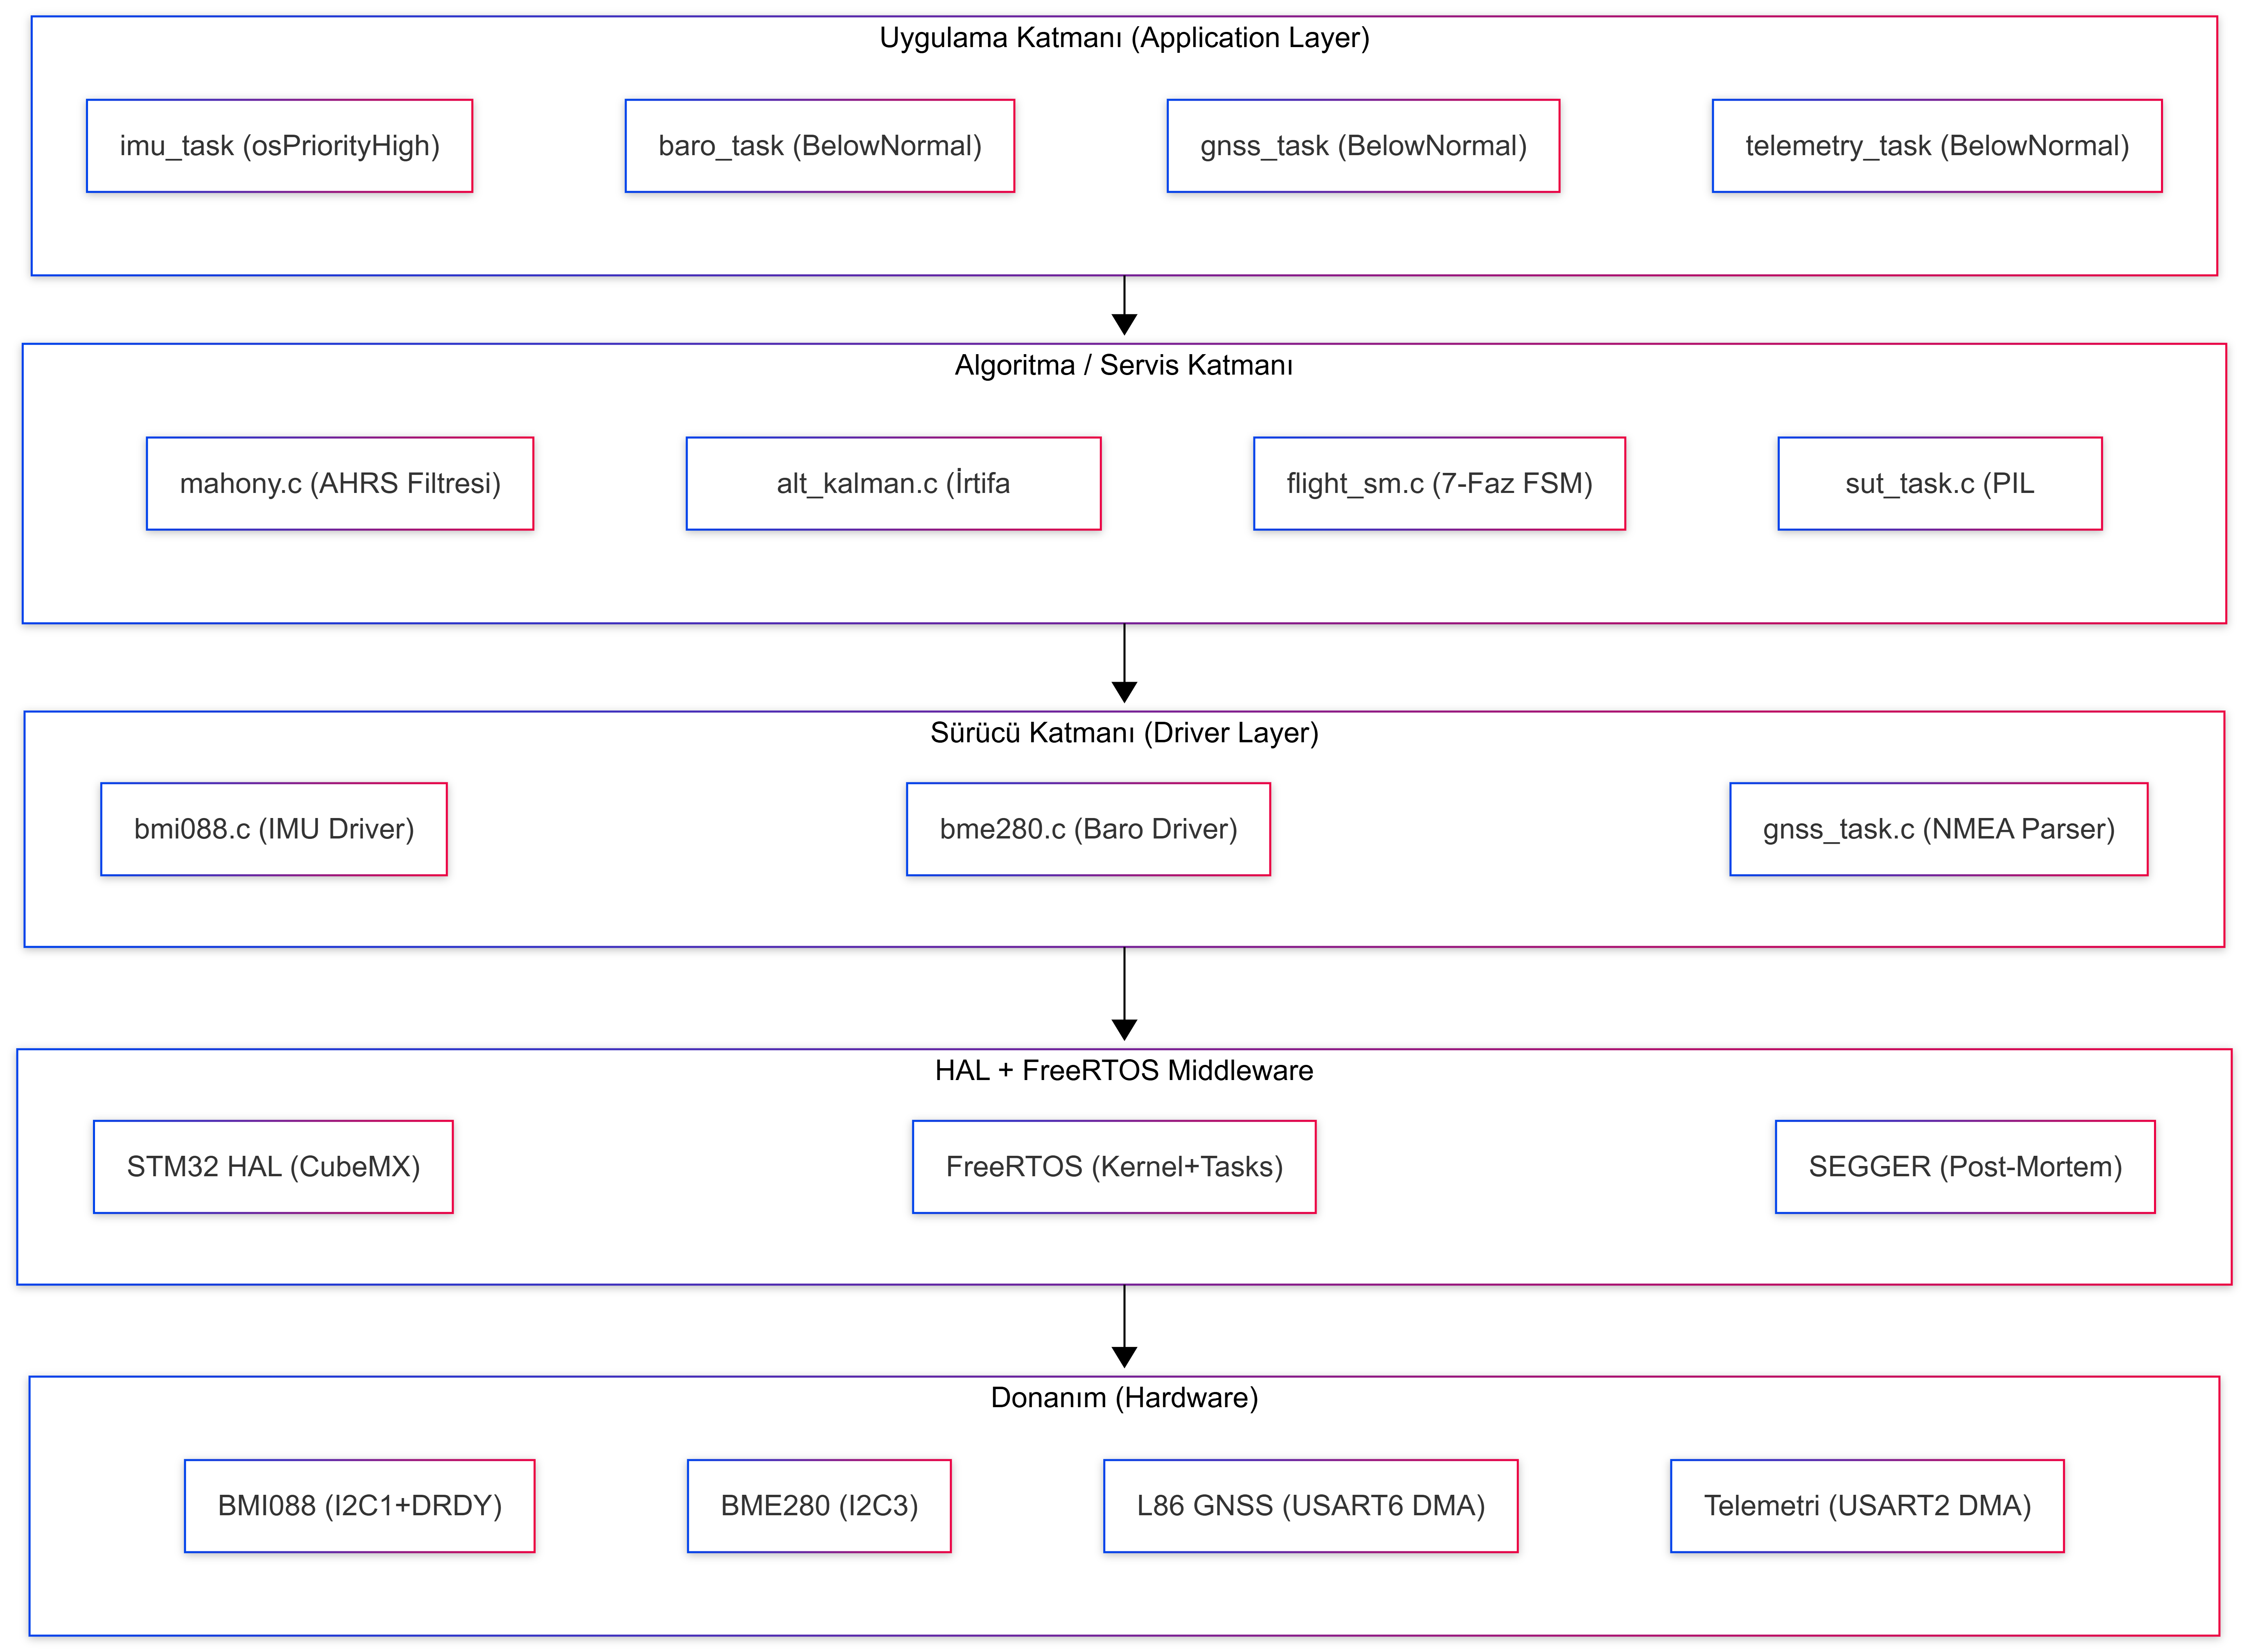
\includegraphics[width=\linewidth,height=0.72\textheight,keepaspectratio]{layered_arch.png}
    \end{column}
    \begin{column}{0.38\textwidth}
      \scriptsize
      Her katman yalnızca altındakiyle konuşur; donanım bağımlılığı izole edilir.
      \begin{itemize}\setlength{\itemsep}{2pt}
        \item \textbf{Uygulama} — imu / baro / gnss / telemetry task
        \item \textbf{Algoritma} — Mahony, Kalman, FSM, SUT
        \item \textbf{Sürücü} — bmi088, bme280, NMEA parser
        \item \textbf{HAL + Middleware} — CubeMX, FreeRTOS, SEGGER
        \item \textbf{Donanım} — BMI088, BME280, L86, USART
      \end{itemize}
      \vspace{2pt}
      \begin{block}{\footnotesize Modülerlik}
        \scriptsize SIT/SUT test katmanları aynı mimariye temiz biçimde eklenir.
      \end{block}
    \end{column}
  \end{columns}
\end{frame}

% ---------------------------------------------------------------
\begin{frame}{Donanım Haritası}{STM32F446 — Cortex-M4 @ 180 MHz, FPU, 512 KB Flash / 128 KB SRAM}
  \centering
  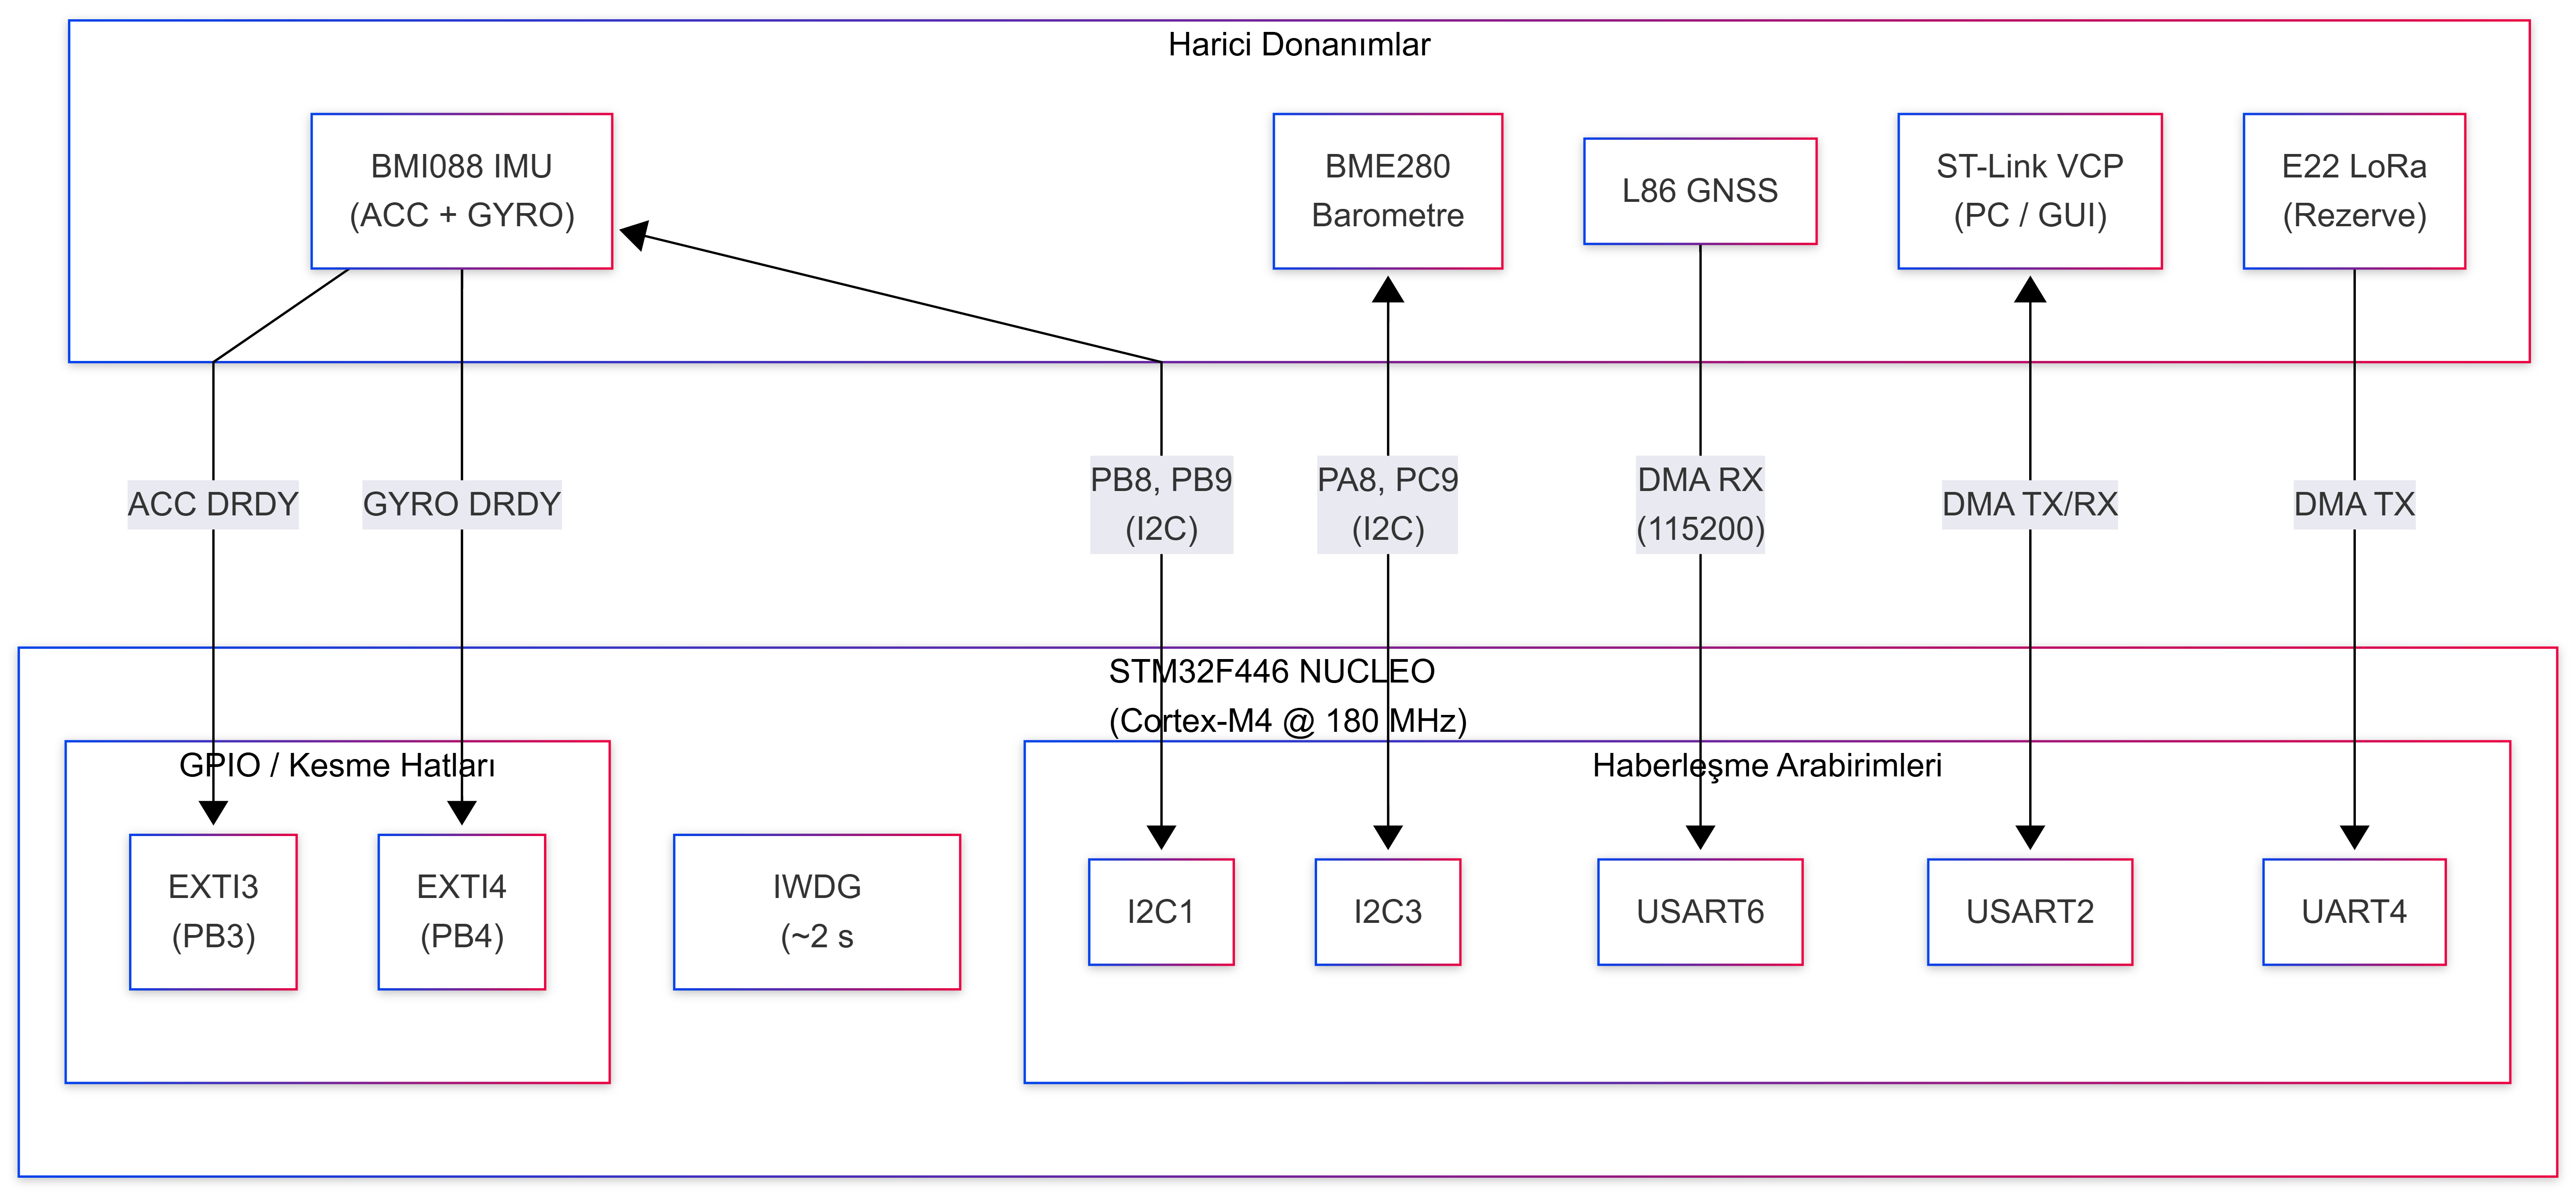
\includegraphics[width=0.92\textwidth,height=0.48\textheight,keepaspectratio]{hw_block.png}
  \par\vspace{3pt}
  \begin{columns}[T]
    \begin{column}{0.42\textwidth}
      \centering\scriptsize
      \begin{tabular}{@{}ll@{}}
        \toprule
        \textbf{Birim} & \textbf{Görev} \\
        \midrule
        I2C1    & BMI088 IMU \\
        I2C3    & BME280 Baro \\
        EXTI3/4 & BMI088 DRDY Kesmesi \\
        USART6  & GNSS (L86) \\
        USART2  & Telemetri / SIT \\
        IWDG    & Donanım Watchdog \\
        \bottomrule
      \end{tabular}
    \end{column}
    \begin{column}{0.58\textwidth}
      \begin{block}{}
        \scriptsize
        \begin{itemize}
          \item \textbf{DMA} — CPU'yu meşgul etmeden veri taşır
          \item \textbf{NVIC + EXTI} — asenkron veri-hazır kesmeleri
          \item \textbf{FPU} — quaternion float işlemleri donanımsal olarak hızlı\\
            \tiny \textit{FPU (Floating Point Unit): kayan nokta işlemlerini yazılımsal\\
            emülasyon yerine donanımda yapar; Mahony/Kalman hesapları\\
            CPU'yu daha az meşgul eder.}
        \end{itemize}
      \end{block}
    \end{column}
  \end{columns}
\end{frame}

% ---------------------------------------------------------------
\begin{frame}{FreeRTOS Görev Modeli}{Sabit öncelikli, birbirini kesebilen dört görev}
  \begin{table}
    \centering\small
    \begin{tabular}{@{}llll@{}}
      \toprule
      \textbf{Görev} & \textbf{Öncelik} & \textbf{Tetikleyici} & \textbf{İşlem / Periyot} \\
      \midrule
      \texttt{imu\_task}       & High        & Donanım kesmesi    & Mahony + snapshot \\
      \texttt{baro\_task}      & BelowNormal & 100 ms periyot     & Kalman + Flight SM \\
      \texttt{gnss\_task}      & BelowNormal & DMA Circular RX    & 1 Hz NMEA parse \\
      \texttt{telemetry\_task} & BelowNormal & İletişim hazır     & 50 Hz UART TX \\
      \bottomrule
    \end{tabular}
  \end{table}
  \vspace{6pt}
  \begin{exampleblock}{Deterministik veri zinciri (IMU)}
    \centering\small
    DRDY Pin $\rightarrow$ EXTI ISR $\rightarrow$ \texttt{xTaskNotifyFromISR} $\rightarrow$
    Görev uyanır $\rightarrow$ DMA başlat $\rightarrow$ DMA-Complete IRQ $\rightarrow$
    Parse $\rightarrow$ Snapshot
  \end{exampleblock}
  \centering\footnotesize
  ISR içinde iş minimumda: sadece bildirim gönderilir, hesaplama göreve devredilir.
\end{frame}

% ---------------------------------------------------------------
\begin{frame}[fragile]{Senkronizasyon Kalıpları}{Bekleme süresini minimuma indiren iki desen}
  \begin{columns}[T]
    \begin{column}{0.5\textwidth}
      \centering
      \textbf{\small ISR $\rightarrow$ Görev: Task Notification}\\[2pt]
      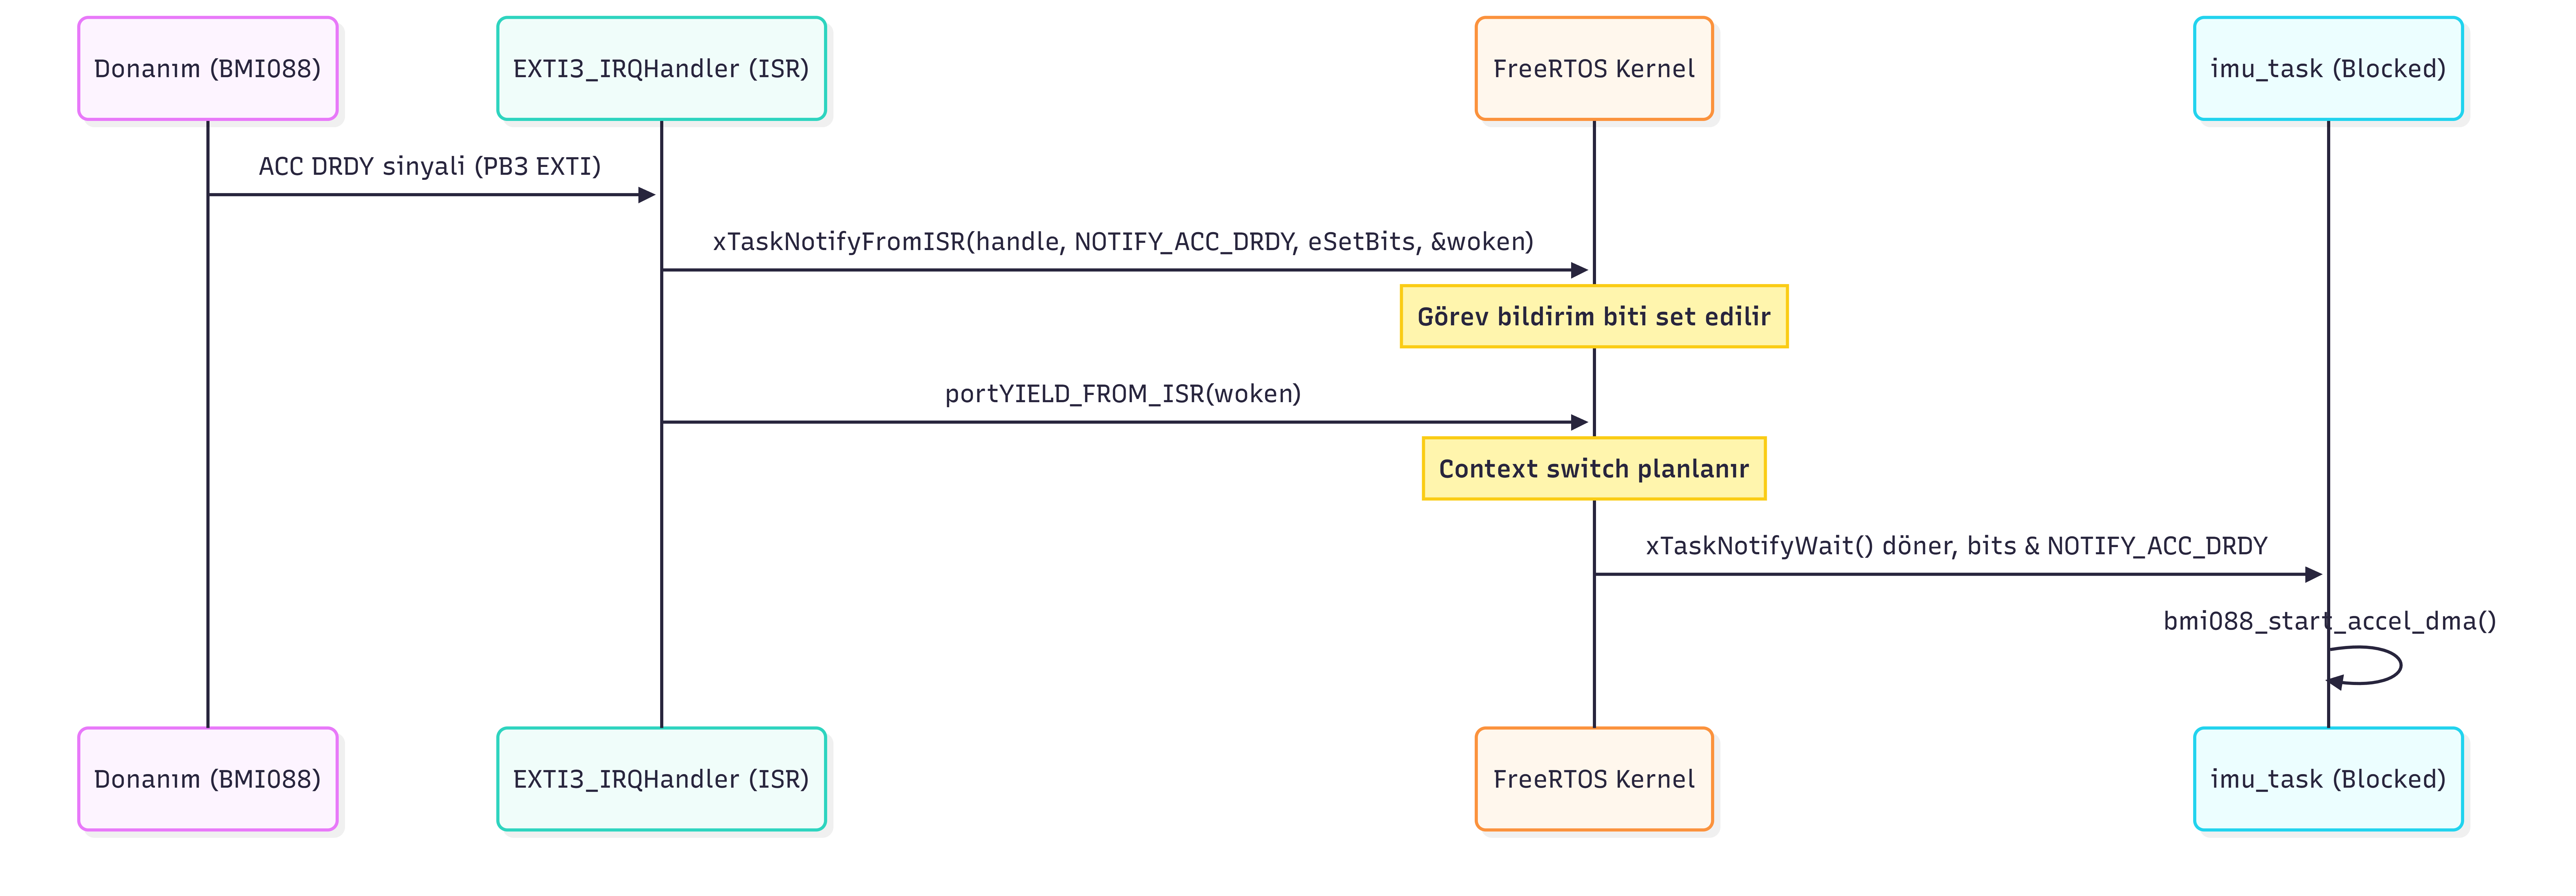
\includegraphics[width=\linewidth,height=0.38\textheight,keepaspectratio]{task_notify.png}
\begin{lstlisting}
void HAL_I2C_MemRxCpltCallback(...)
{
  BaseType_t woken = pdFALSE;
  xTaskNotifyFromISR(s_handle,
      NOTIFY_DMA_DONE, eSetBits, &woken);
  portYIELD_FROM_ISR(woken);
}
\end{lstlisting}
    \end{column}
    \begin{column}{0.5\textwidth}
      \centering
      \textbf{\small Görev $\rightarrow$ Görev: Snapshot Queue}\\[2pt]
      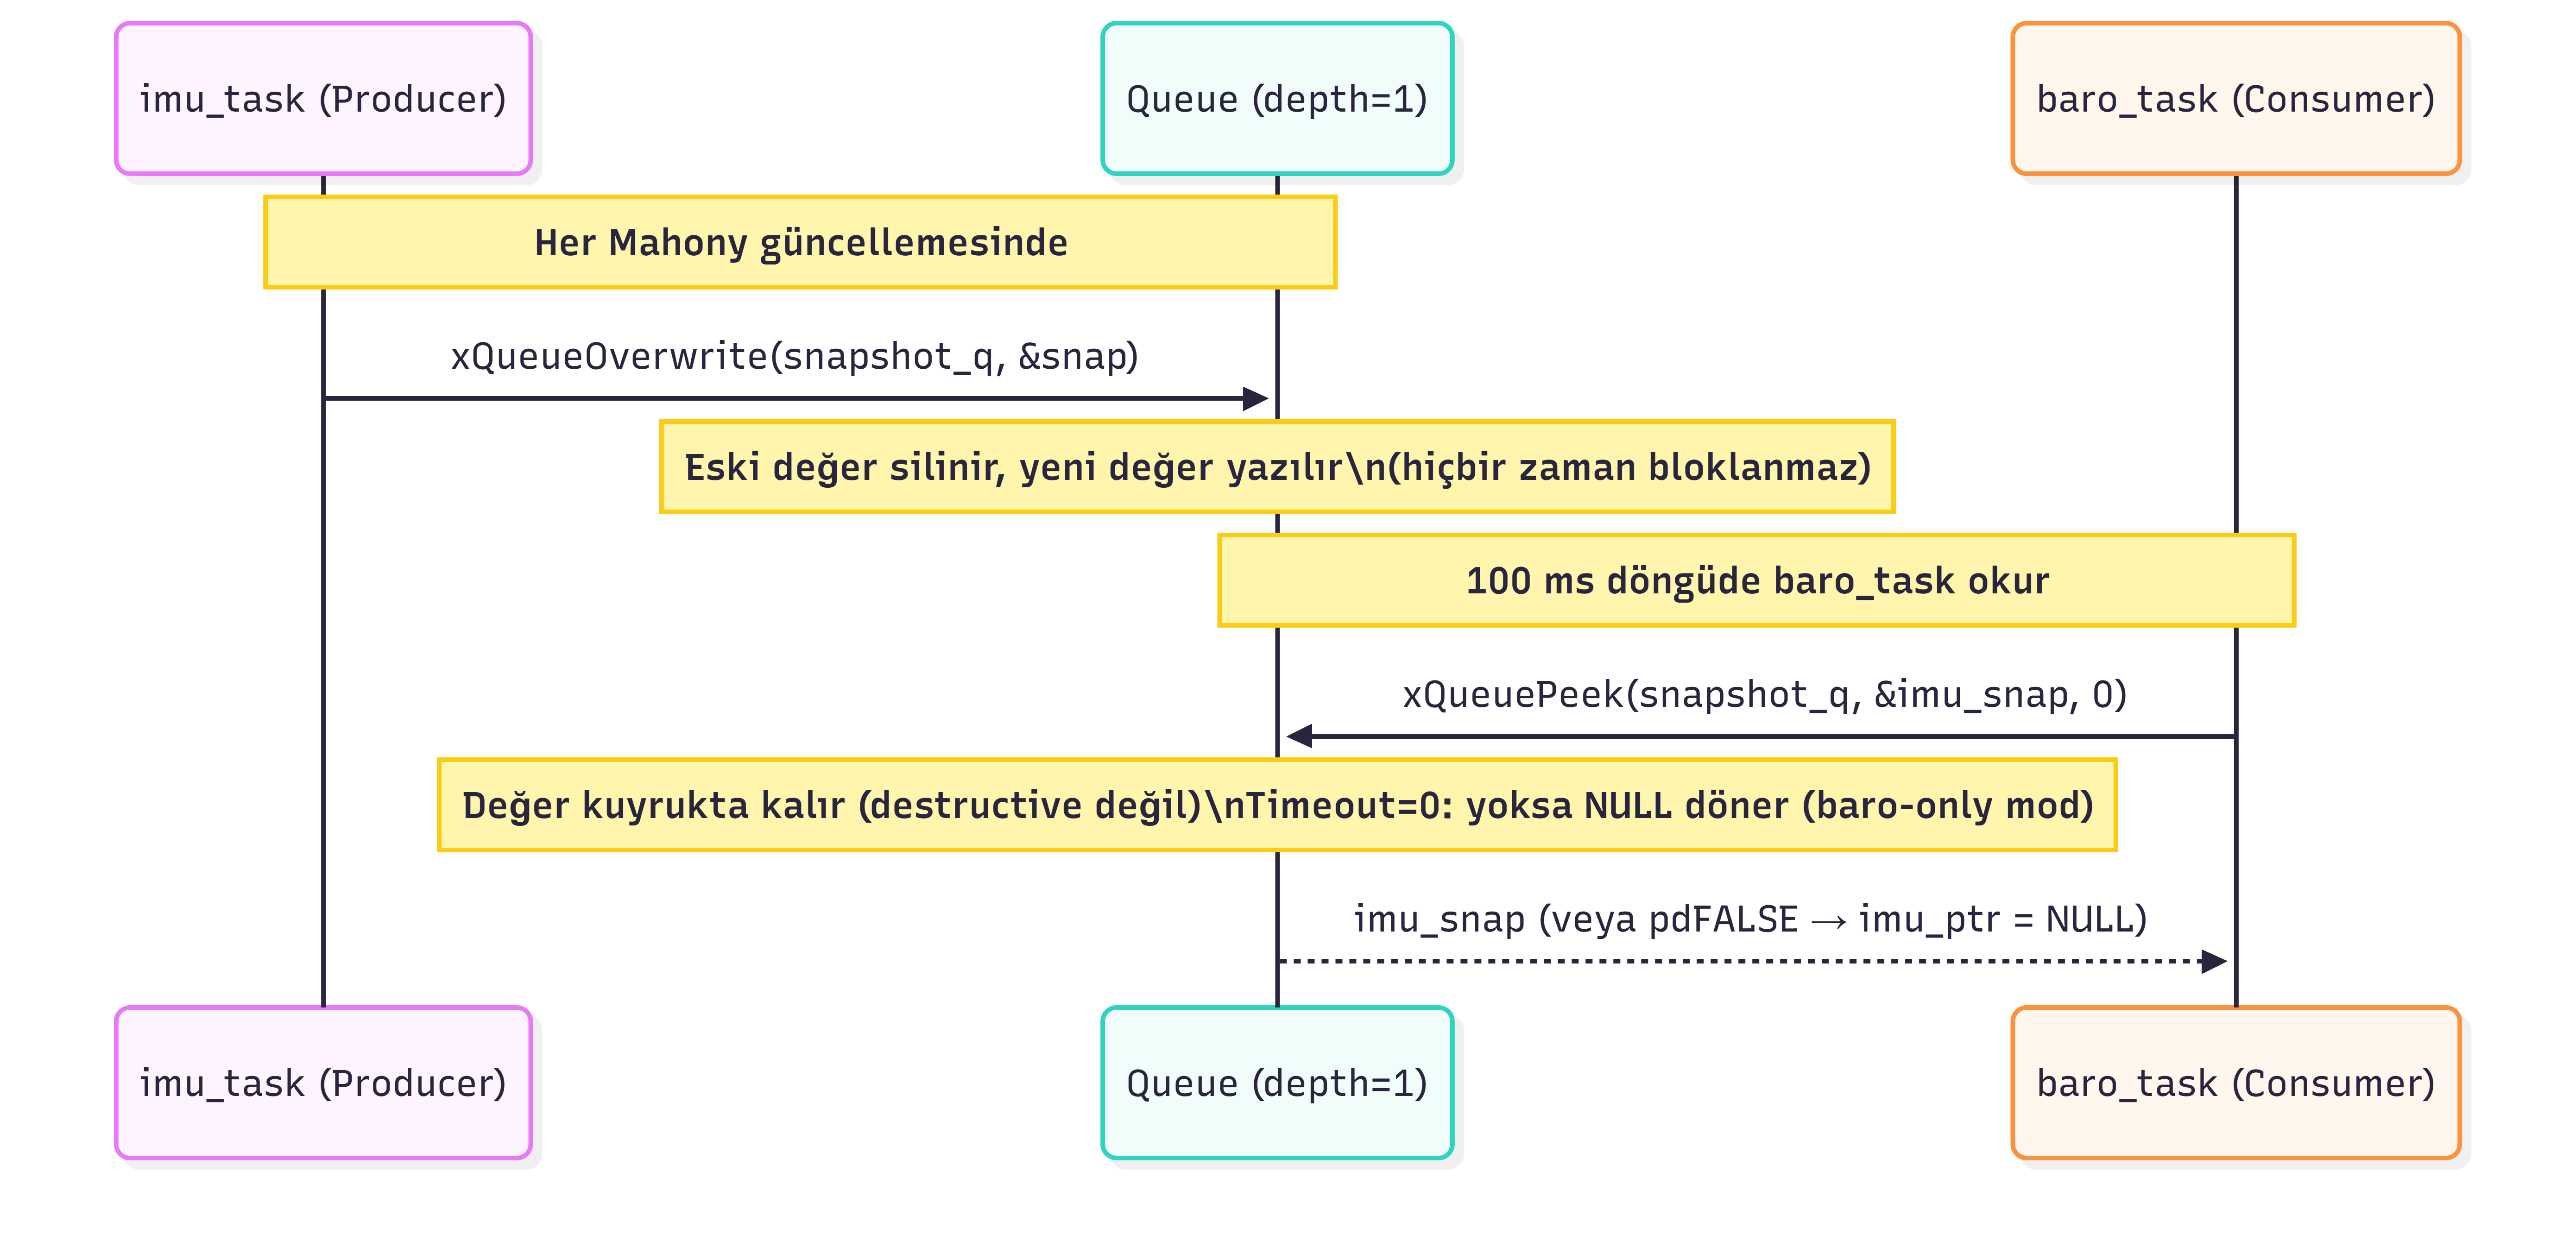
\includegraphics[width=\linewidth,height=0.44\textheight,keepaspectratio]{snapshot_queue.png}
      \vspace{2pt}
      \begin{block}{\footnotesize Derinliği 1 kuyruk (mailbox)}
        \scriptsize
        \begin{itemize}
          \item \texttt{xQueueOverwrite} — üretici hep son veriyi yazar
          \item \texttt{xQueuePeek} — tüketici eksiltmeden okur
          \item Tek sahipli, atomik, gereksiz tamponlama yok
        \end{itemize}
      \end{block}
    \end{column}
  \end{columns}
\end{frame}

% =================================================================
% BÖLÜM 3 — SENSÖR FÜZYONU VE UÇUŞ ALGORİTMASI
% =================================================================
\section{Sensör Füzyonu ve Uçuş Algoritması}

% ---------------------------------------------------------------
\begin{frame}{IMU Veri İşleme Hattı ve Mahony AHRS}{Yönelim kestirimi (Roll / Pitch / Yaw)}
  \centering
  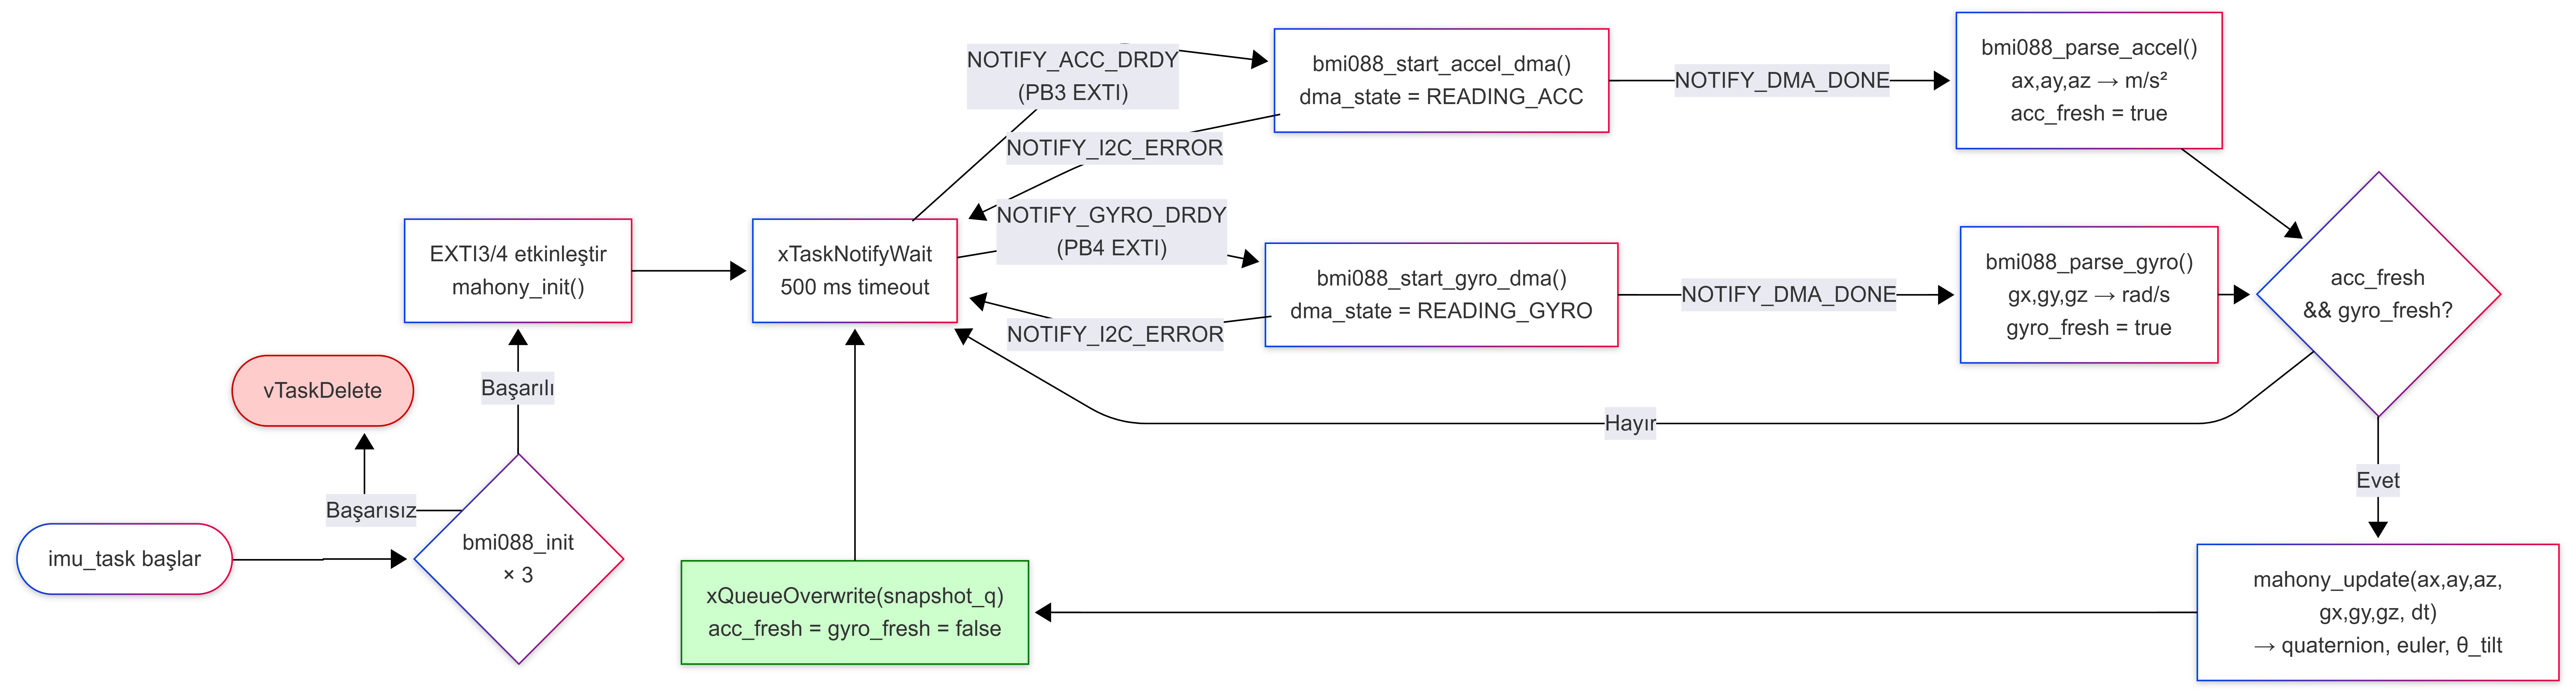
\includegraphics[width=\textwidth,height=0.46\textheight,keepaspectratio]{imu_pipeline.png}
  \par\vspace{2pt}
  \begin{columns}[T]
    \begin{column}{0.36\textwidth}
      \begin{block}{\tiny Neden füzyon?}
        \tiny İvmeölçer titreşimde \textbf{gürültülü}; jiroskop zamanla \textbf{kayar}. İkisinin güçlü yönü birleştirilir.
      \end{block}
    \end{column}
    \begin{column}{0.64\textwidth}
      \begin{exampleblock}{\tiny Mahony AHRS — Nasıl Çalışır?}
        \tiny
        \textbf{AHRS} = Attitude \& Heading Ref. System (Roll/Pitch/Yaw)\\[1pt]
        \textbf{1.} Jiro $\rightarrow$ açısal hız $\rightarrow$ quaternion güncelle\quad
        \textbf{2.} İvmeölçer $\rightarrow$ yerçekimi ref. $\rightarrow$ hata hesapla\quad
        \textbf{3.} PI $\rightarrow$ düzelt\\[1pt]
        \textit{Jiro hız bilgisi verir; ivmeölçer ``kayıyorsun, düzelt'' der.}\\[1pt]
        \textbf{$k_p$} = düzeltme hızı ($k_p{\uparrow}$ titreşime duyarlı, $k_p{\downarrow}$ yavaş)\enspace
        \textbf{$k_i$} = bias düzeltmesi\\
        SIT'te statik açı salınımına bakılarak ayarlandı.\enspace Yakınsama: \textbf{2--3 s}.
      \end{exampleblock}
    \end{column}
  \end{columns}
\end{frame}

% ---------------------------------------------------------------
\begin{frame}{Yükseklik Kalman Filtresi}{Baro + IMU füzyonu ile gürültüden arınmış irtifa}
  \centering
  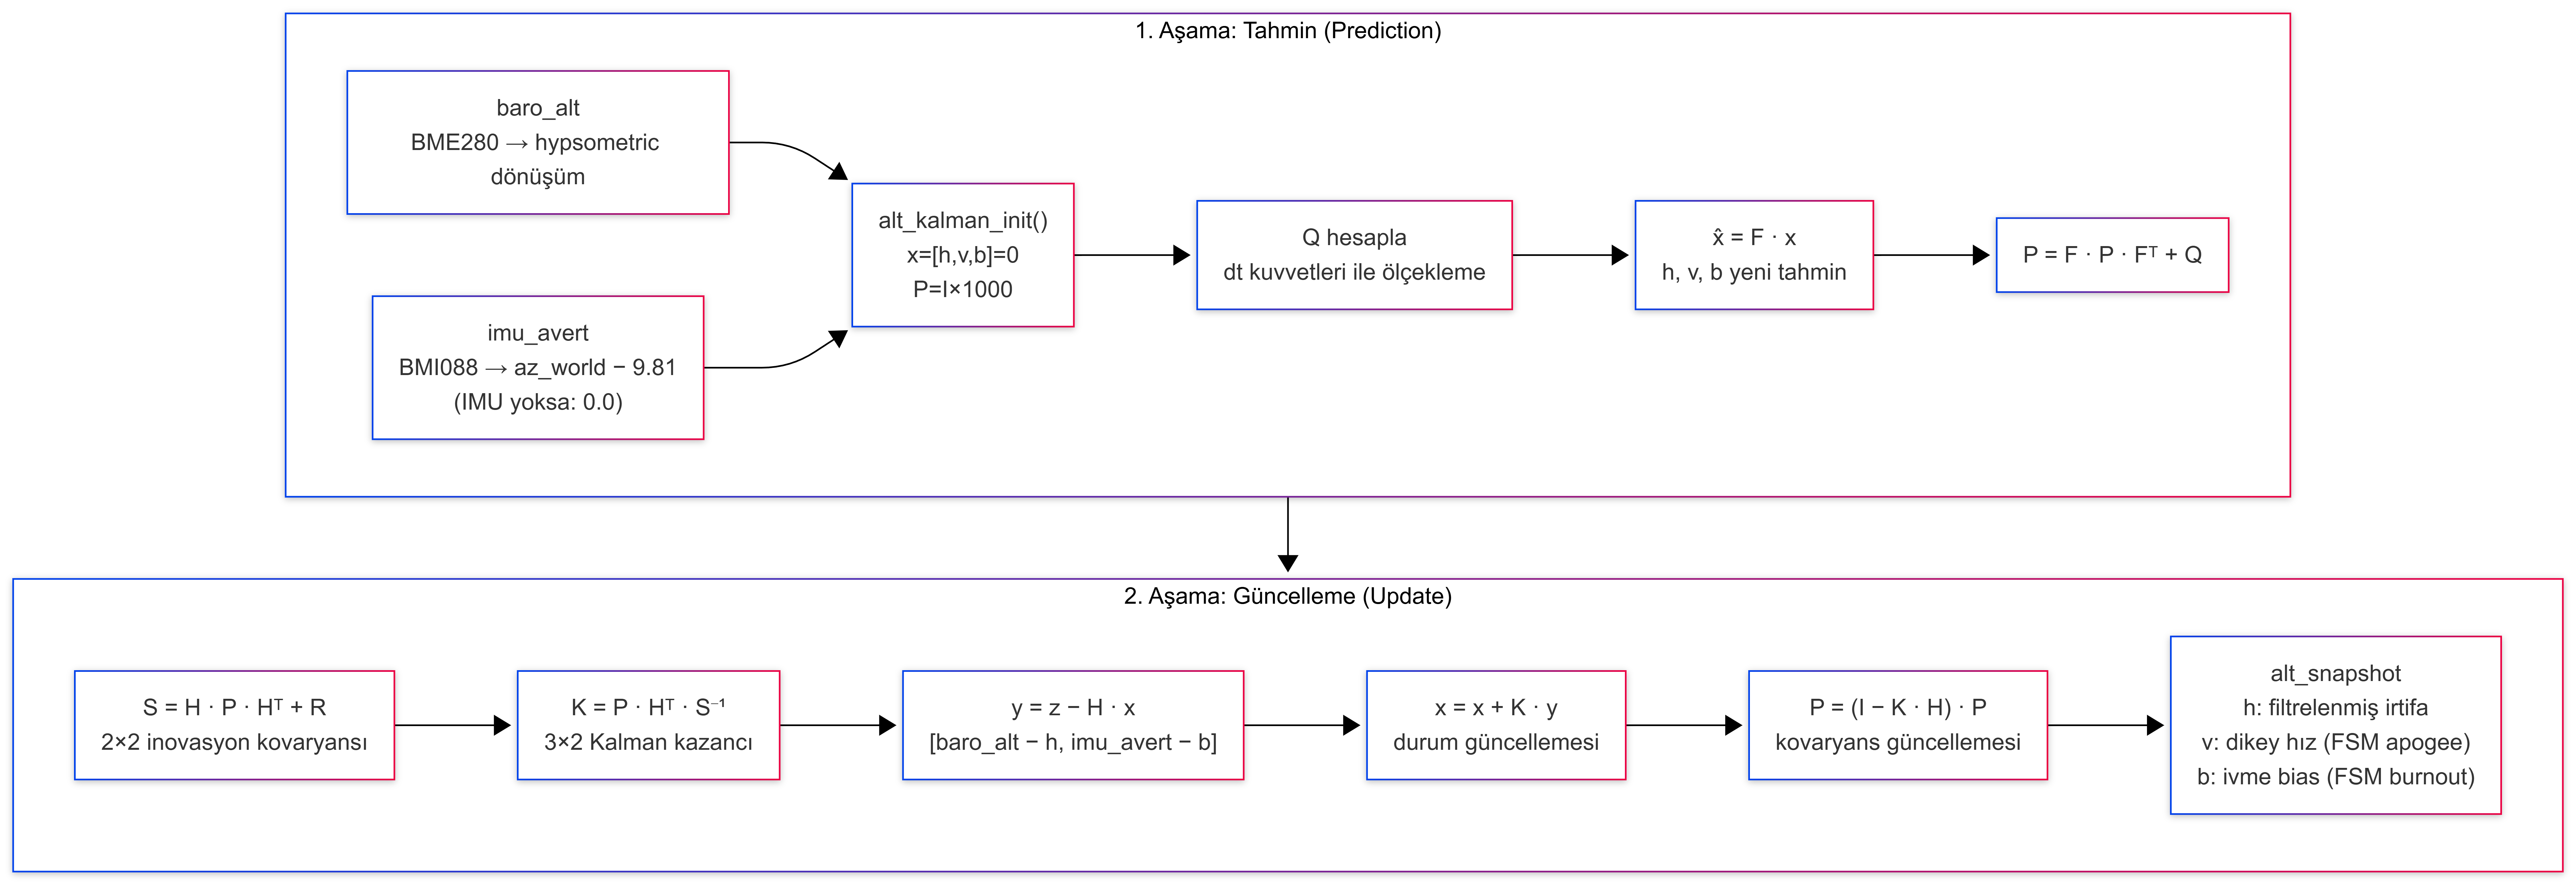
\includegraphics[width=\textwidth,height=0.44\textheight,keepaspectratio]{kalman.png}
  \par\vspace{2pt}
  \begin{columns}[T]
    \begin{column}{0.40\textwidth}
      \begin{block}{\tiny 3-durumlu kestirim}
        \tiny \textbf{[irtifa,\ hız,\ ivme-bias]}\\
        Baro: yavaş ama mutlak ref.\\
        IMU: hızlı ama kayma var\\
        Kalman $\rightarrow$ güvenilir \textbf{hız} $\rightarrow$ doğru apogee
      \end{block}
      \vspace{1pt}
      \begin{alertblock}{\tiny Q ve R}
        \tiny
        \textbf{R} = ölçüm gürültüsü (baro varyansı ölçüldü)\\
        \textbf{Q} = süreç gürültüsü (model sapması)\\
        Q${\downarrow}$ sensöre güven / Q${\uparrow}$ modele güven
      \end{alertblock}
    \end{column}
    \begin{column}{0.60\textwidth}
      \begin{exampleblock}{\tiny Nasıl Çalışır? — Predict \& Update}
        \tiny
        \textbf{Predict:} fizik modeli ile sonraki durumu tahmin et\\
        \quad irtifa $+{=}$ hız$\times$dt,\enspace hız $+{=}$ ivme$\times$dt\\[2pt]
        \textbf{Update:} baro ölçümü gelince tahmini düzelt\\[2pt]
        \textbf{R} = baroya ne kadar güvenilsin?\\
        \quad R${\uparrow}$ $\rightarrow$ az ağırlık\enspace/\enspace R${\downarrow}$ $\rightarrow$ çok ağırlık\\
        \quad Baro gürültülü $\Rightarrow$ R yüksek tutuldu.
      \end{exampleblock}
    \end{column}
  \end{columns}
\end{frame}

% ---------------------------------------------------------------
\begin{frame}{Uçuş Durum Makinesi — 7 Faz}{If-else spagettisi yerine izlenebilir FSM}
  \begin{columns}[c]
    \begin{column}{0.58\textwidth}
      \centering
      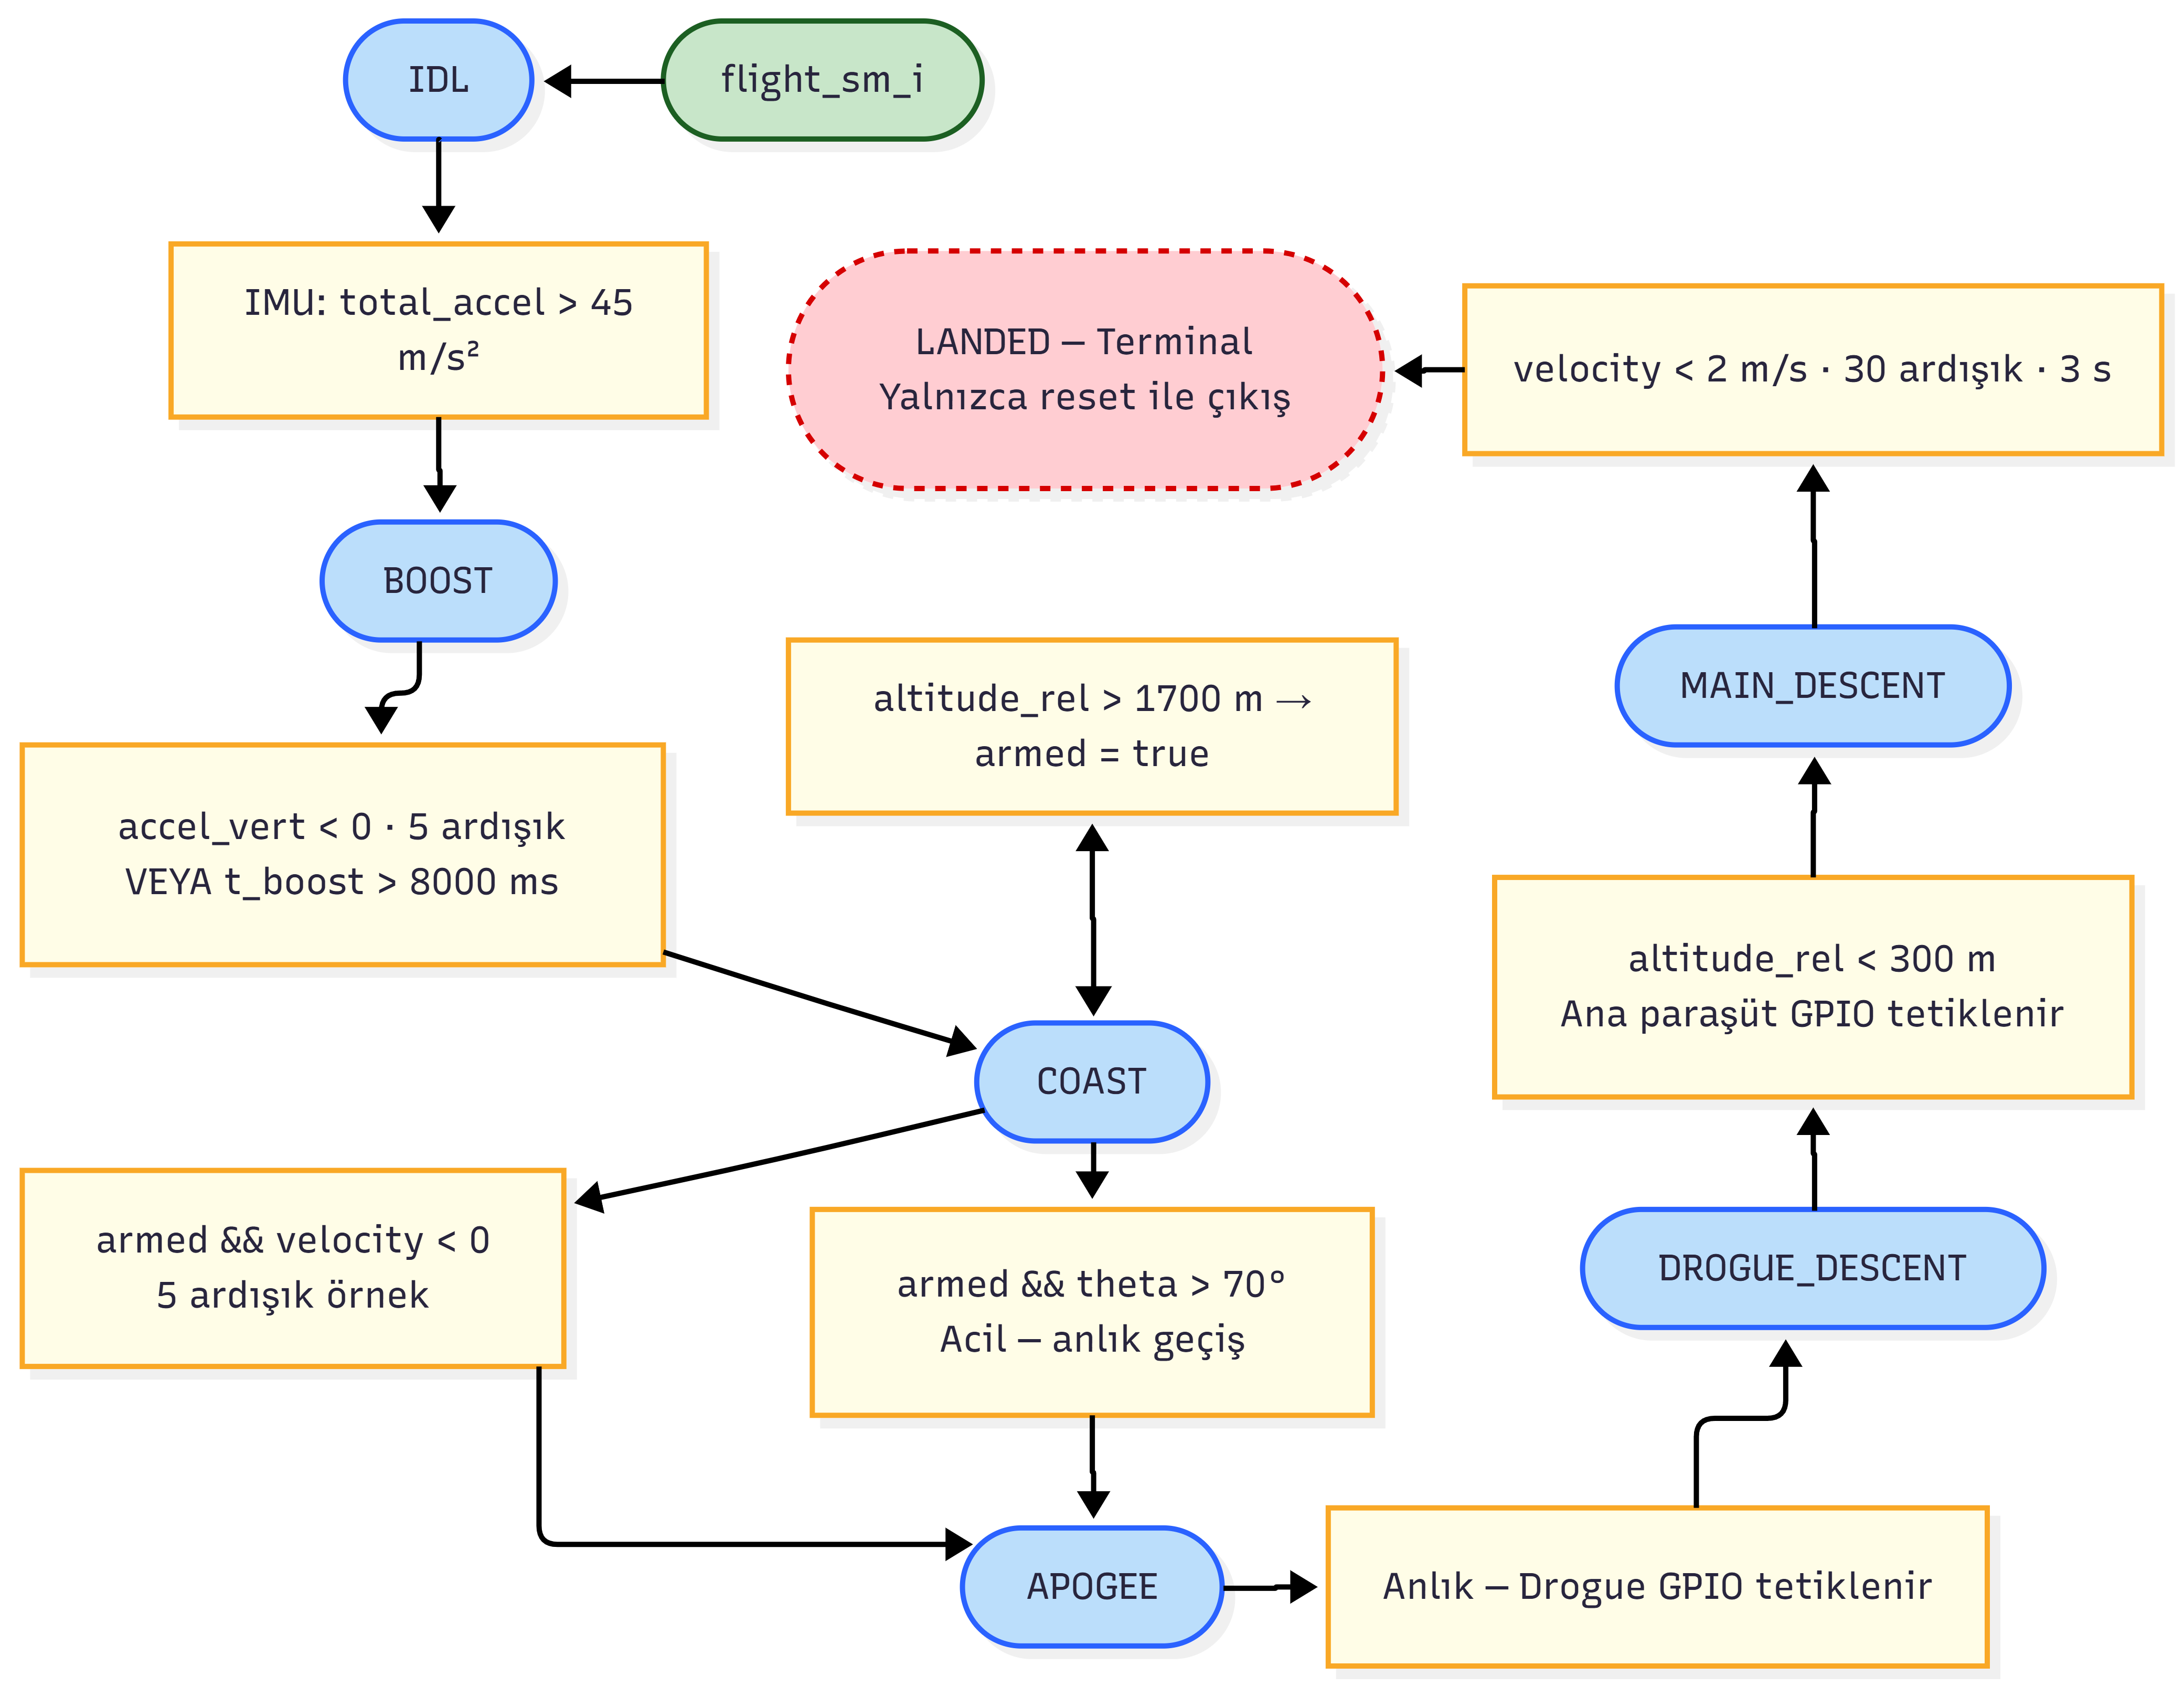
\includegraphics[width=\linewidth,height=0.64\textheight,keepaspectratio]{flight_fsm.png}
    \end{column}
    \begin{column}{0.42\textwidth}
      \scriptsize
      \textbf{IDLE} $\rightarrow$ \textbf{BOOST} $\rightarrow$ \textbf{COAST} $\rightarrow$
      \textbf{APOGEE} $\rightarrow$ \textbf{DROGUE} $\rightarrow$ \textbf{MAIN} $\rightarrow$ \textbf{LANDED}
      \vspace{4pt}
      \begin{alertblock}{\footnotesize Çift güvenlikli apogee}
        \scriptsize
        \begin{itemize}
          \item \textbf{Hız bazlı:} Kalman dikey hızı $<$ 0
          \item \textbf{Tilt bazlı:} Pitch açısı $>$ 70$^\circ$
        \end{itemize}
        Biri tetiklenince Drogue paraşütü açılır.
      \end{alertblock}
      \begin{itemize}
        \item BOOST: ivme $>$ 45 m/s$^2$
        \item MAIN: irtifa $<$ 300 m
        \item LANDED: hız $<$ 2 m/s
      \end{itemize}
    \end{column}
  \end{columns}
\end{frame}

% ---------------------------------------------------------------
\begin{frame}{Güvenilirlik Mekanizmaları}{Kilitlenmeye ve sensör arızasına karşı koruma}
  \begin{columns}[T]
    \begin{column}{0.5\textwidth}
      \begin{block}{Donanımsal / yazılımsal kalkanlar}
        \scriptsize
        \begin{itemize}\setlength{\itemsep}{3pt}
          \item \textbf{IWDG watchdog} ($\sim$2 s)\\
            \tiny Donanım sayacı geri sayar; yazılım 2 sn içinde sıfırlamazsa CPU reset atar.
            Baro görevi her 100 ms'de bir besler — donma olursa otomatik kurtarma.
          \item \textbf{Stack overflow koruması}\\
            \tiny Her FreeRTOS task'ının ayrı stack'i var. \texttt{configCHECK\_FOR\_STACK\_OVERFLOW=2}:
            FreeRTOS her context-switch'te stack dolgusunu kontrol eder; taşma varsa hook çağrılır.
          \item \textbf{Fatal handler} $\rightarrow$ \texttt{NVIC\_SystemReset()}\\
            \tiny Hata durumunda sonsuz döngüde kalmak yerine sistemi yeniden başlatır.
            IWDG + reset = sistem kendi kendine toparlanabilir.
        \end{itemize}
      \end{block}
    \end{column}
    \begin{column}{0.5\textwidth}
      \begin{exampleblock}{Baro-only ``degraded'' mod}
        \footnotesize IMU başlamazsa sistem \textbf{kaybolmaz, uçmaya devam eder}:
        \scriptsize
        \begin{tabular}{@{}lll@{}}
          \toprule
          \textbf{Özellik} & \textbf{IMU var} & \textbf{IMU yok} \\
          \midrule
          BOOST tespiti & ivme & baro hızı \\
          Kalman girdisi & dikey ivme & 0 \\
          Tilt apogee & aktif & pasif \\
          Hız apogee & aktif & \textbf{aktif} \\
          \bottomrule
        \end{tabular}
      \end{exampleblock}
      \centering\scriptsize
      IMU sürücüsü 3 deneme başarısız olursa görev silinir, sistem baro moduyla devam eder.
    \end{column}
  \end{columns}
\end{frame}

% =================================================================
% BÖLÜM 4 — TEST, DOĞRULAMA VE BULGULAR
% =================================================================
\section{Test, Doğrulama ve Bulgular}

% ---------------------------------------------------------------
\begin{frame}{Test Metodolojisi: SIT ve SUT}{İki katmanlı doğrulama — fiziksel roket olmadan}
  \begin{columns}[c]
    \begin{column}{0.42\textwidth}
      \begin{block}{\small SIT — Sensör İzleme Testi}
        \scriptsize
        \emph{Donanım / sürücü} doğrulaması.
        \begin{itemize}
          \item Gerçek sensör $\rightarrow$ STM32 $\rightarrow$ Python GUI
          \item DMA / I2C / USART yolları test edilir
          \item Statik test: Z ekseni $\approx -9.81$ m/s$^2$
        \end{itemize}
      \end{block}
      \vspace{6pt}
      \begin{exampleblock}{\small SUT — Sentetik Uçuş Testi (PIL)}
        \scriptsize
        \emph{Algoritma / FSM} doğrulaması.
        \begin{itemize}
          \item \textbf{Processor-in-the-Loop}
          \item PC, RocketPy verisini UART'tan yollar
          \item STM32 Mahony + Kalman + FSM çalıştırır
        \end{itemize}
      \end{exampleblock}
    \end{column}
    \begin{column}{0.58\textwidth}
      \centering
      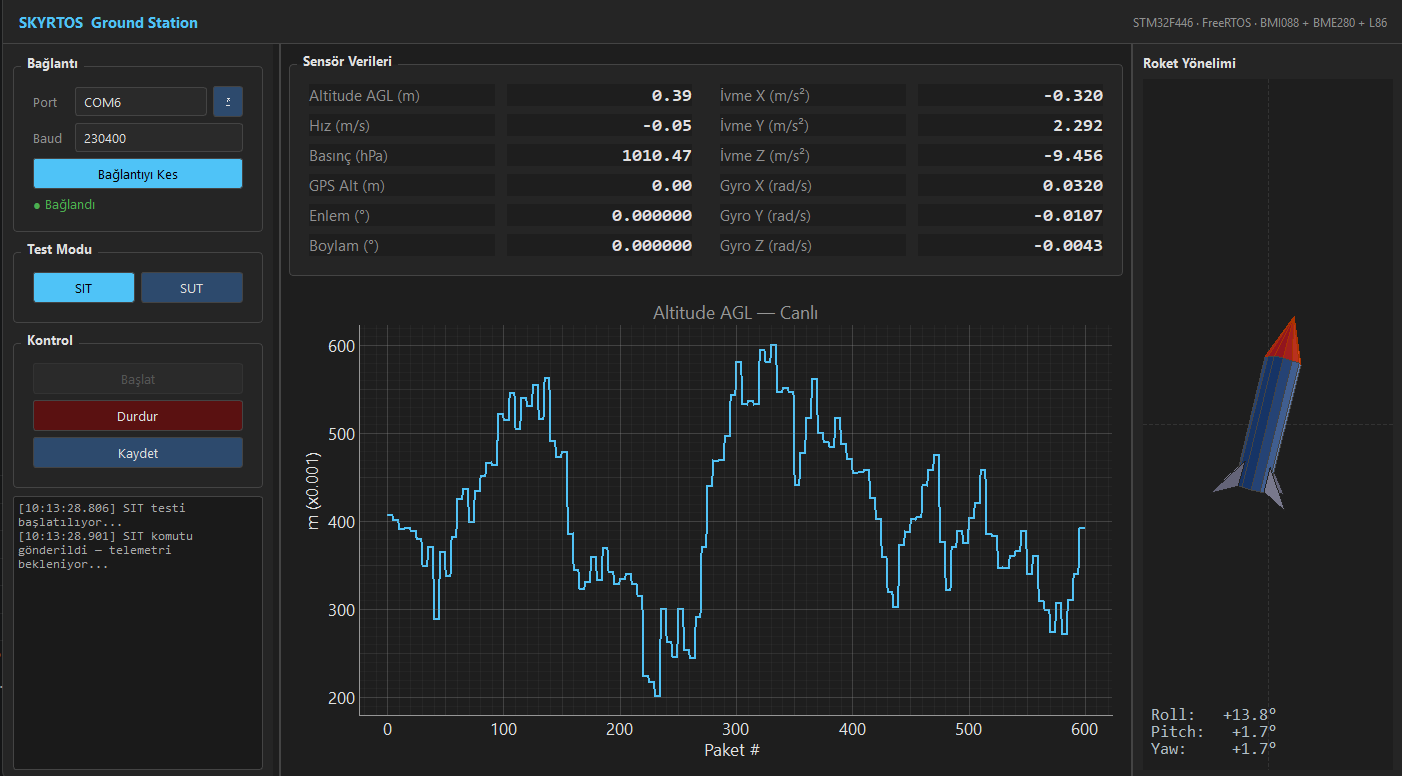
\includegraphics[width=\linewidth,height=0.74\textheight,keepaspectratio]{sit_gui.png}\\[2pt]
      {\scriptsize SIT arayüzü — canlı telemetri ve 3D yönelim}
    \end{column}
  \end{columns}
\end{frame}

% ---------------------------------------------------------------
\begin{frame}{SUT — RocketPy ile Sentetik Uçuş (PIL)}{Gerçek uçuş koşullarına eşdeğer referans veri}
  \begin{columns}[c]
    \begin{column}{0.44\textwidth}
      \centering
      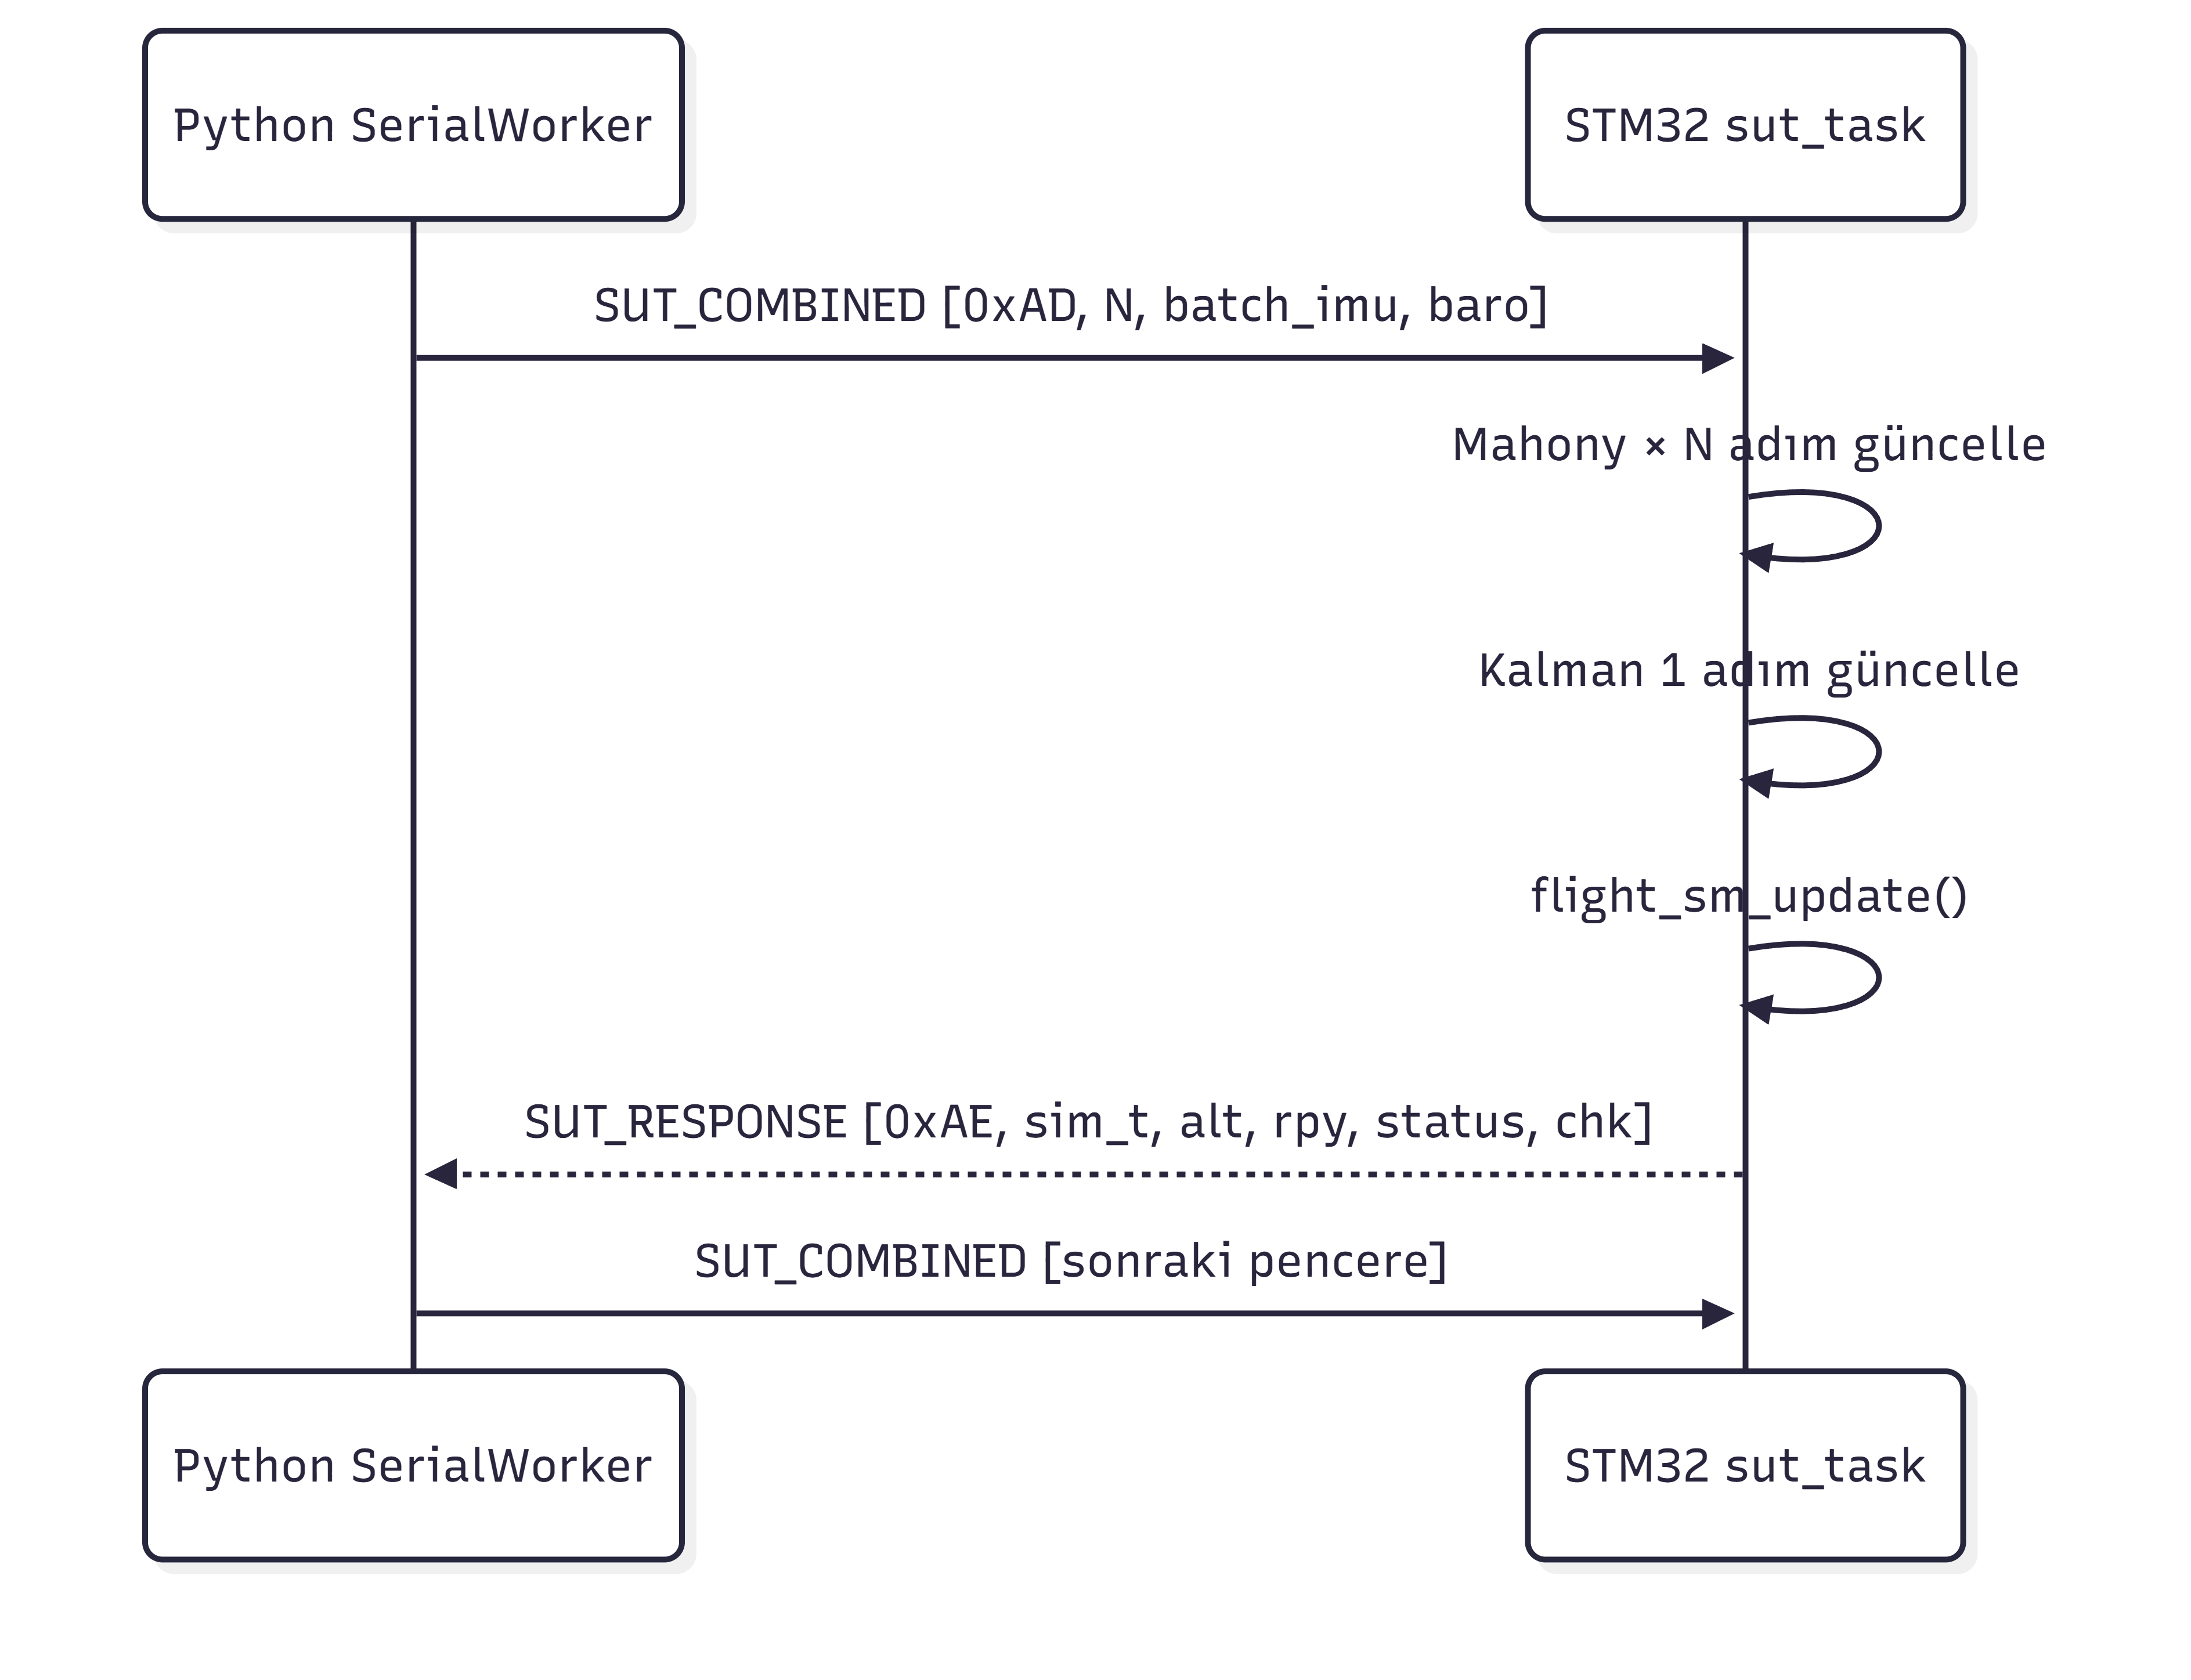
\includegraphics[width=\linewidth,height=0.56\textheight,keepaspectratio]{sut_arch.png}\\[2pt]
      {\scriptsize Processor-in-the-Loop akış şeması}
    \end{column}
    \begin{column}{0.56\textwidth}
      \centering
      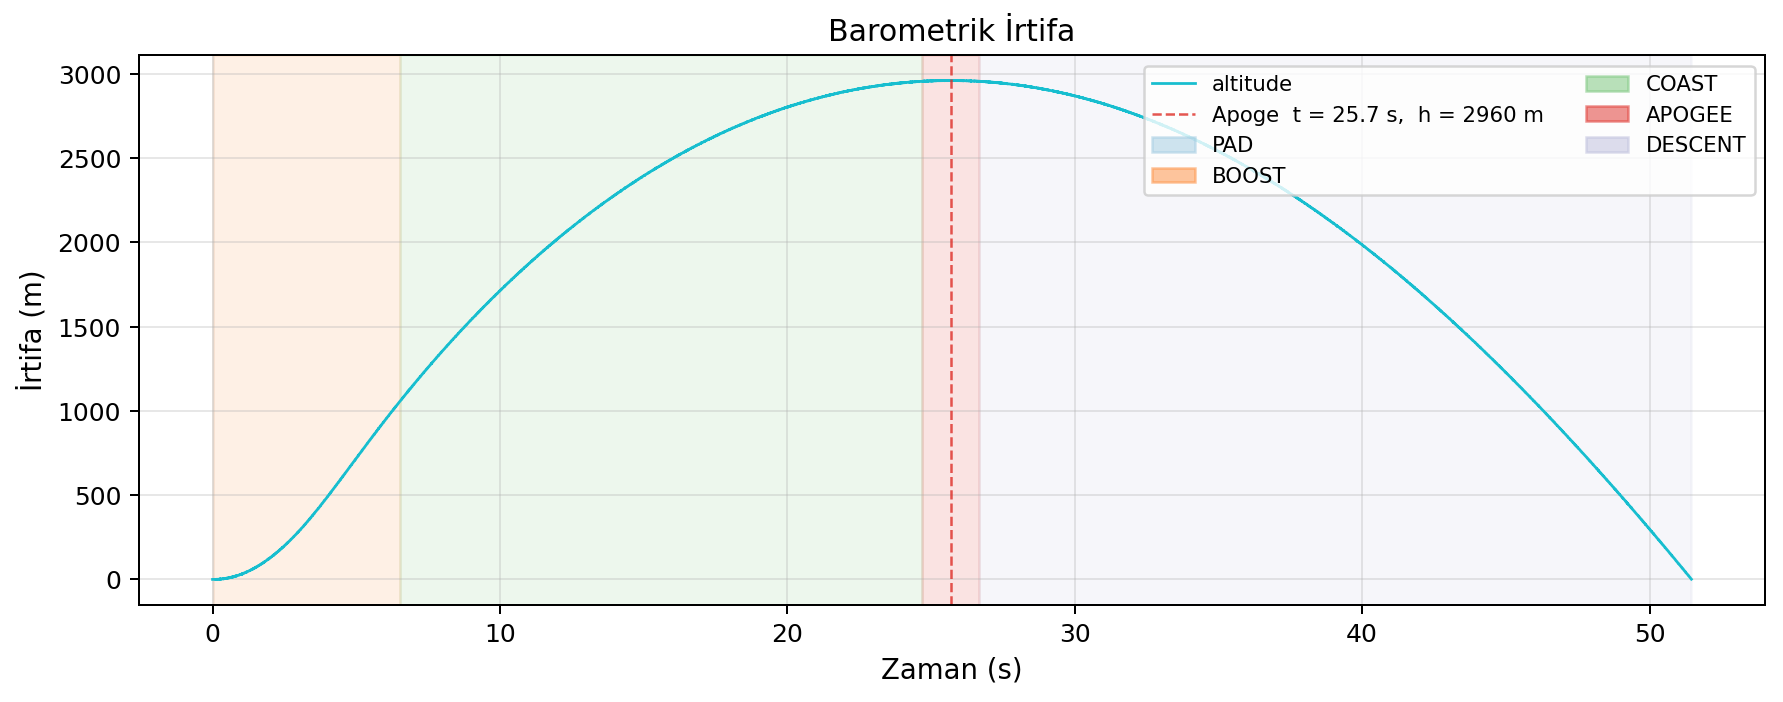
\includegraphics[width=\linewidth,height=0.46\textheight,keepaspectratio]{sim_altitude.png}\\[4pt]
      \begin{exampleblock}{}
        \centering\scriptsize
        RocketPy simülasyon verisi UART üzerinden STM32'ye aktarılır;\\
        Mahony + Kalman + FSM \textbf{gerçek zamanlı} çalışır ve\\
        tüm FSM faz geçişleri doğrulanır.
      \end{exampleblock}
    \end{column}
  \end{columns}
\end{frame}

% ---------------------------------------------------------------
\begin{frame}{Sonuç 1 — Kalman Filtresi}{Ham baro vs. filtrelenmiş irtifa}
  \begin{columns}[c]
    \begin{column}{0.5\textwidth}
      \centering
      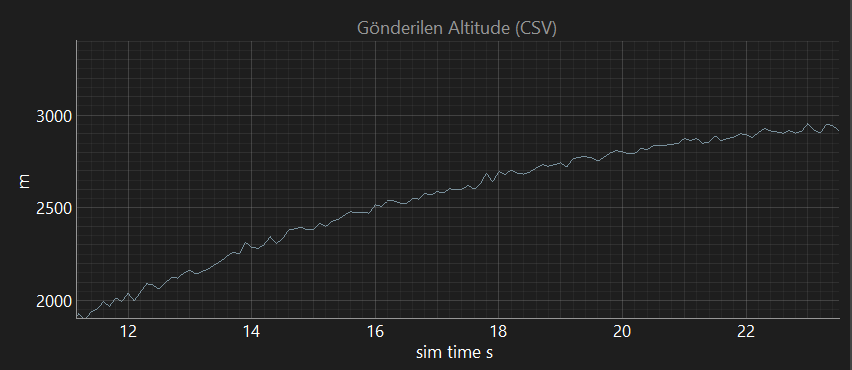
\includegraphics[width=\linewidth,height=0.58\textheight,keepaspectratio]{kalman_result_nonfilter.png}\\[2pt]
      {\scriptsize \textbf{Filtresiz} — Ham barometre çıkışı}
    \end{column}
    \begin{column}{0.5\textwidth}
      \centering
      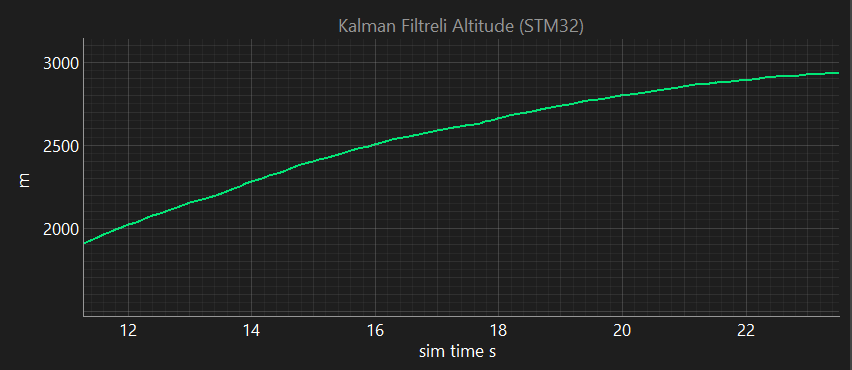
\includegraphics[width=\linewidth,height=0.58\textheight,keepaspectratio]{kalman_result_filter.png}\\[2pt]
      {\scriptsize \textbf{Filtrelenmiş} — 3-durumlu Kalman çıkışı}
    \end{column}
  \end{columns}
  \vspace{4pt}
  \begin{exampleblock}{}
    \centering\scriptsize
    Kalman filtresi baro gürültüsünü baskılarken ivmeölçer füzyonu ile
    \textbf{hız ve irtifa tahminini} kararlı hâle getirir —
    apogee tespiti ve FSM geçişleri bu çıktı üzerinden çalışır.
  \end{exampleblock}
\end{frame}

% ---------------------------------------------------------------
\begin{frame}{SUT Testi — Tamamlanmış Uçuş}{FSM faz geçişleri ve 3D yönelim}
  \centering
  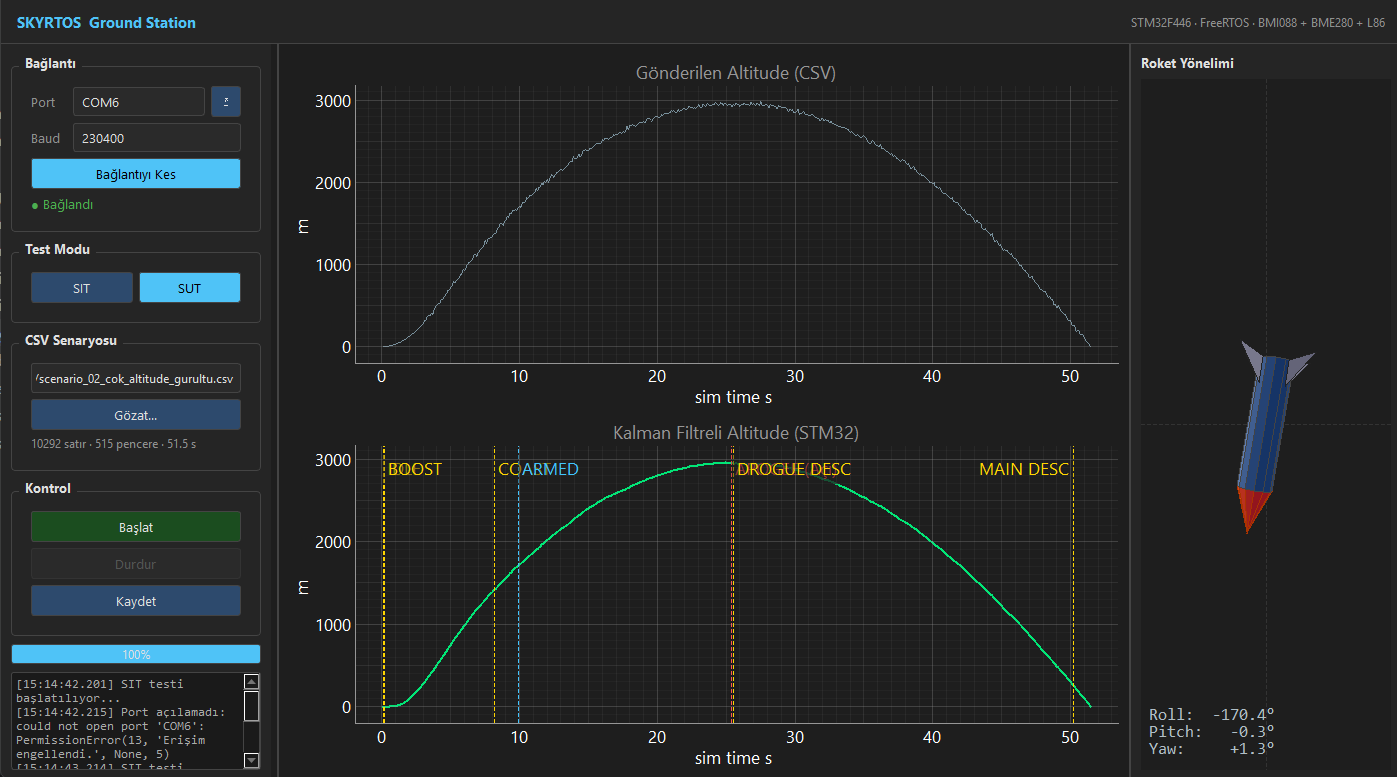
\includegraphics[width=\textwidth,height=0.78\textheight,keepaspectratio]{sut_gui.png}
\end{frame}


% ---------------------------------------------------------------
\begin{frame}{Preemption Kanıtı}{Yüksek öncelikli IMU, çalışan BARO görevini keserek işlemciyi devraldı}
  \centering
  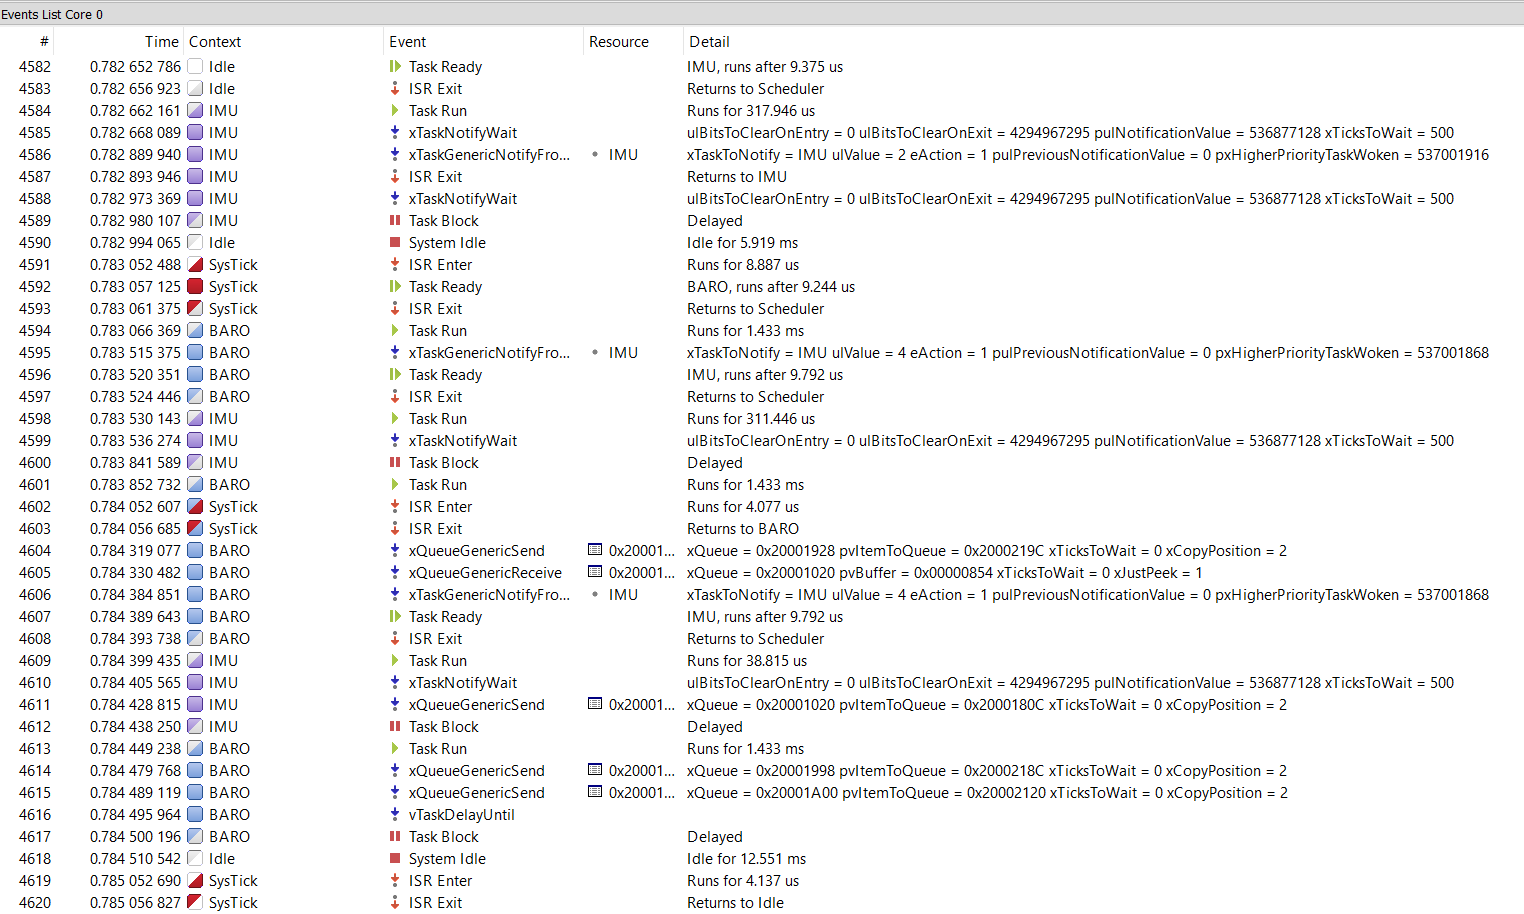
\includegraphics[width=\textwidth,height=0.78\textheight,keepaspectratio]{event_list_imu_baro.png}
\end{frame}

% ---------------------------------------------------------------
\begin{frame}{Sonuç 3 — IMU Mahony Füzyon Kararlılığı}{300 saniyelik durağan drift testi}
  \begin{columns}[c]
    \begin{column}{0.5\textwidth}
      \centering
      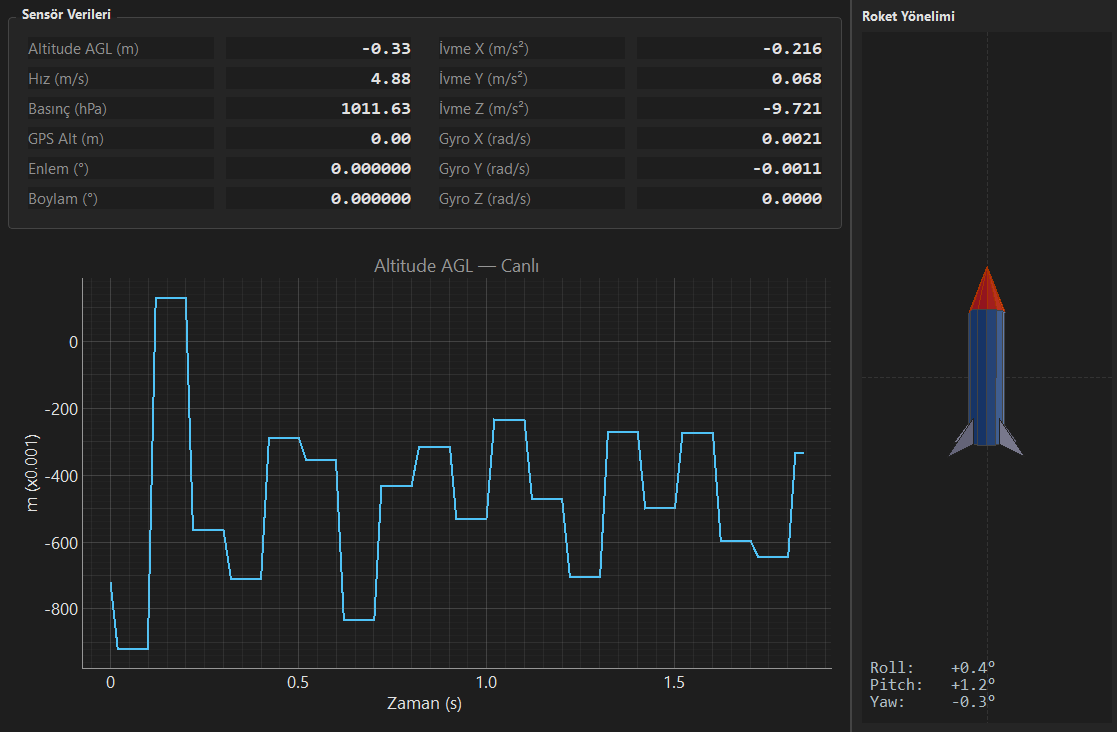
\includegraphics[width=\linewidth,height=0.55\textheight,keepaspectratio]{imu_1s.png}\\[2pt]
      {\scriptsize \textbf{1. saniye} — başlangıç referansı}
    \end{column}
    \begin{column}{0.5\textwidth}
      \centering
      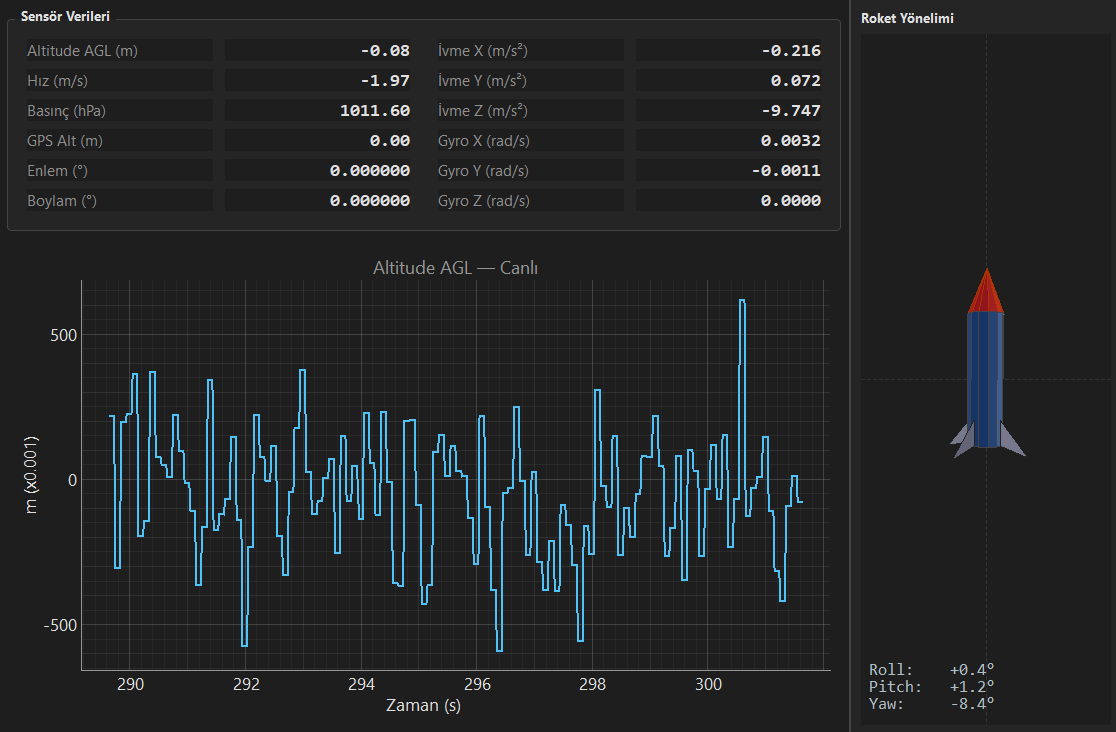
\includegraphics[width=\linewidth,height=0.55\textheight,keepaspectratio]{imu_300s.png}\\[2pt]
      {\scriptsize \textbf{300. saniye} — Yaw drift gözlemi}
    \end{column}
  \end{columns}
  \vspace{2pt}
  \begin{columns}[T]
    \begin{column}{0.5\textwidth}
      \begin{block}{\scriptsize Roll \& Pitch}
        \tiny 300 saniye boyunca \textbf{kayma yok}.\\
        Mahony yerçekimi vektörünü referans alır $\rightarrow$ ivmeölçer her adımda düzeltir.
      \end{block}
    \end{column}
    \begin{column}{0.5\textwidth}
      \begin{alertblock}{\scriptsize Yaw — Neden Drift?}
        \tiny Mahony'nin Yaw için referans vektörü \textbf{yok}.\\
        Manyetometre olsaydı manyetik kuzey referans verirdi.\\
        Sadece jiroskop entegrali var $\rightarrow$ her örnekte küçük hata birikir $\rightarrow$ drift.\\[1pt]
        \textit{Uçuşta sorun değil: $\sim$60 sn uçuşta drift apogee tespitini etkilemiyor.}
      \end{alertblock}
    \end{column}
  \end{columns}
\end{frame}

% =================================================================
% BÖLÜM 5 — SONUÇ VE ÖNERİLER
% =================================================================
\section{Sonuç ve Öneriler}

% ---------------------------------------------------------------
% Metrik tablosu slaytı
\begin{frame}{Ölçülen Başarım Metrikleri}{SEGGER SystemView post-mortem + CMake build çıktısı}
  \centering
  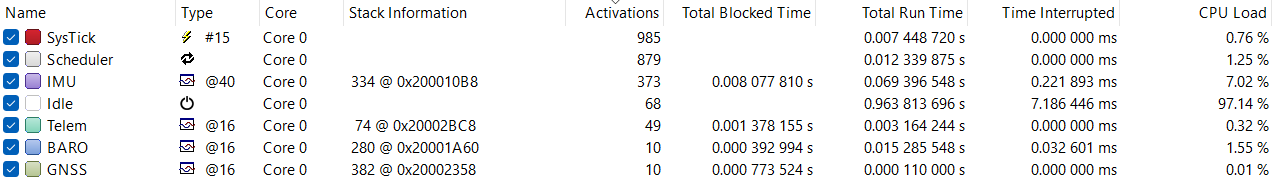
\includegraphics[width=\textwidth,height=0.48\textheight,keepaspectratio]{context.png}
  \par\vspace{6pt}
  \begin{columns}[T]
    \begin{column}{0.5\textwidth}
      \begin{exampleblock}{\small CPU \& Görev Verimi}
        \scriptsize
        \begin{itemize}
          \item İşlemci zamanının \textbf{\color{izuBordo}\%97.14}'ü Idle — sistem rahat çalışıyor
          \item IMU en yoğun görev: \textbf{373 Hz} aktivasyon, \textbf{\%7.02} CPU
          \item Baro + Telemetri + GNSS toplam: \textbf{$<$ 2\%}
          \item Stack taşması \& veri kaybı: \textbf{Sıfır}
        \end{itemize}
      \end{exampleblock}
    \end{column}
    \begin{column}{0.5\textwidth}
      \begin{block}{\small Bellek \& Doğrulama}
        \scriptsize
        \begin{itemize}
          \item Flash kullanımı: \textbf{77.9 KB} / 512 KB \enspace(\textbf{\%14.9})
          \item RAM kullanımı (yazılım): \textbf{26.8 KB} / 128 KB \enspace(\textbf{\%20.4})
          \item SUT tamamlama süresi: \textbf{51.5 sn}
          \item Tüm FSM faz geçişleri RocketPy ile doğrulandı
        \end{itemize}
      \end{block}
    \end{column}
  \end{columns}
\end{frame}

% Sonuç ve öneriler slaytı
\begin{frame}{Sonuç ve Gelecek Çalışmalar}
  \begin{columns}[T]
    \begin{column}{0.5\textwidth}
      \begin{exampleblock}{Başarılan hedefler}
        \footnotesize
        \begin{itemize}
          \item STM32F446 üzerinde hard real-time FreeRTOS uçuş yazılımı
          \item DMA + kesme tabanlı asenkron veri toplama
          \item Mahony AHRS + 3-durumlu Kalman füzyonu
          \item 7-fazlı FSM ile hatasız faz geçişleri
          \item IWDG + degraded mod ile güvenilirlik
          \item SIT / SUT (PIL) ile RocketPy doğrulaması
        \end{itemize}
      \end{exampleblock}
    \end{column}
    \begin{column}{0.5\textwidth}
      \begin{block}{Gelecek çalışmalar}
        \footnotesize
        \begin{itemize}
          \item \textbf{Gyro kalibrasyonu} — IDLE'da bias ölçümü
          \item \textbf{Fiziksel fırlatma} — saha doğrulaması
          \item \textbf{LoRa (E22)} — UART4 hattı donanımda hazır
          \item \textbf{EKF + kara kutu} — SD log ile gelişmiş filtre
        \end{itemize}
      \end{block}
    \end{column}
  \end{columns}
  \vspace{4pt}
  \begin{alertblock}{\centering Değişmez prensip}
    \centering\small
    Önce güvenilir ve anlaşılır çalışan basit sistem $\rightarrow$ sonra genişletme.
  \end{alertblock}
\end{frame}


% Teşekkür slaytı
\begin{frame}[plain]
  \begin{tikzpicture}[remember picture, overlay]
    \fill[izuDark] (current page.north west) rectangle (current page.south east);
    \node[anchor=south east, inner sep=0.04\paperwidth] at (current page.south east)
      {
\includegraphics[height=0.14\paperheight]{izu_logo}};
  \end{tikzpicture}
  \vfill
  \centering
  {\color{white}\Huge\bfseries Dinlediğiniz için teşekkürler}\par
  \vspace{0.4cm}
  \textcolor{izuGold}{\rule{10em}{0.8pt}}\par
  \vspace{0.3cm}
  {\color{white!70!izuDark}\large\insertauthor}\par
  \vspace{0.1cm}
  {\color{white!50!izuDark}\small\insertinstitute}
  \vfill
\end{frame}


\end{document}
